% !TeX spellcheck = en_US
% !TeX encoding = UTF-8
\documentclass[a4paper]{article}
\usepackage{graphics, graphicx}
\usepackage{fancyvrb, enumerate}
\usepackage{amsmath, amssymb, amscd, amsfonts}
\usepackage{geometry}
\usepackage{multirow}
\usepackage{url}
\usepackage{listings, listing}
\usepackage{color}
\usepackage{mathptmx}
\usepackage[numberedbib]{apacite}
\usepackage[style=iso]{datetime2}
\usepackage{csvsimple, booktabs}

\geometry
{
    top = 20mm,
    bottom = 20mm,
    left = 20mm,
    right = 20mm
}

\title{Periodontitis}
\author{
    Seunghoon Kim
    \and
    Jaewoong Lee
    \and
    Semin Lee
}
\date{\today}

\begin{document}
   	\maketitle
    \newpage

    \tableofcontents
    \listoftables
    \listoffigures
    \newpage

    \section{Introduction}
        \subsection{Microbiome}
            Microbiome is consist of microbiota, the micro-organisms which live inside and on humans \cite{microbiome1}. Microbiome is also about $10^{13}$ micro-organisms whose which collective genome \cite{microbiome2}.

            \begin{figure}[p]
                \centering
                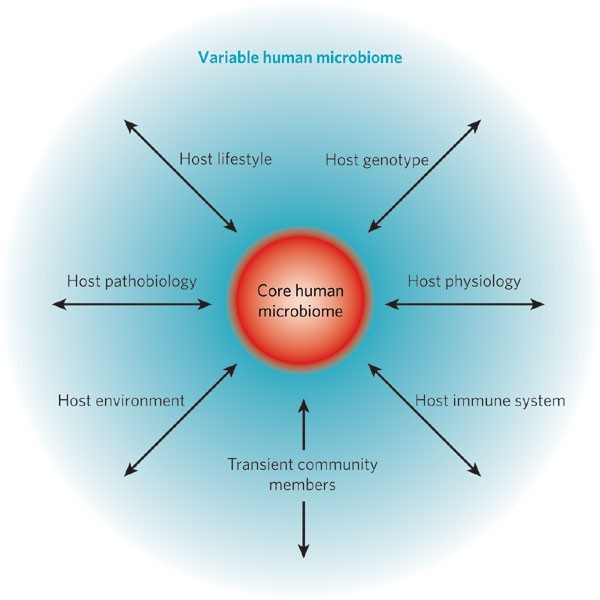
\includegraphics[width=0.4 \linewidth]{figures/microbiome.jpg}
                \caption{Concept of a Core Human Microbiome \protect\cite{microbiome1}}
                \label{fig:microbiome-concept}
            \end{figure}

        \subsection{Ribosomal RNA}
            Ribosomal RNA (rRNA) is well-known as a key to phylogeny \cite{rRNA1}.

        \subsection{16S rRNA Gene Sequencing}

        \subsection{Periodontitis}
            Periodontitis is an inflammatory conditions which effecting periodontium, tissues  which surround and support teeth. Major components of periodontitis are clinical attachment loss and bone loss \cite{periodontitis1}. Previous study found risk factors of periodontitis such as smoking, diabetes, genetic factors and host response \cite{periodontitis2}.

    \section{Materials}
        \subsection{16S rRNA Gene Sequencing}

            \begin{itemize}
                \item 100 Healthy samples
                \item 50 Chronic Early Periodontitis Sample
                \item 50 Chronic Moderate Periodontitis Sample
                \item 50 Chronic Severe Periodontitis Sample
            \end{itemize}

    \section{Methods}
        \subsection{QIIME2 Workflow}
            QIIME2 is a capable, expandable and distributed microbiome analysis package with transparent analysis \cite{qiime1, qiime2}. A theoretic overview of QIIME2 workflow is shown as figure \ref{fig:qiime-workflow}.

            \begin{figure}[p]
                \centering
                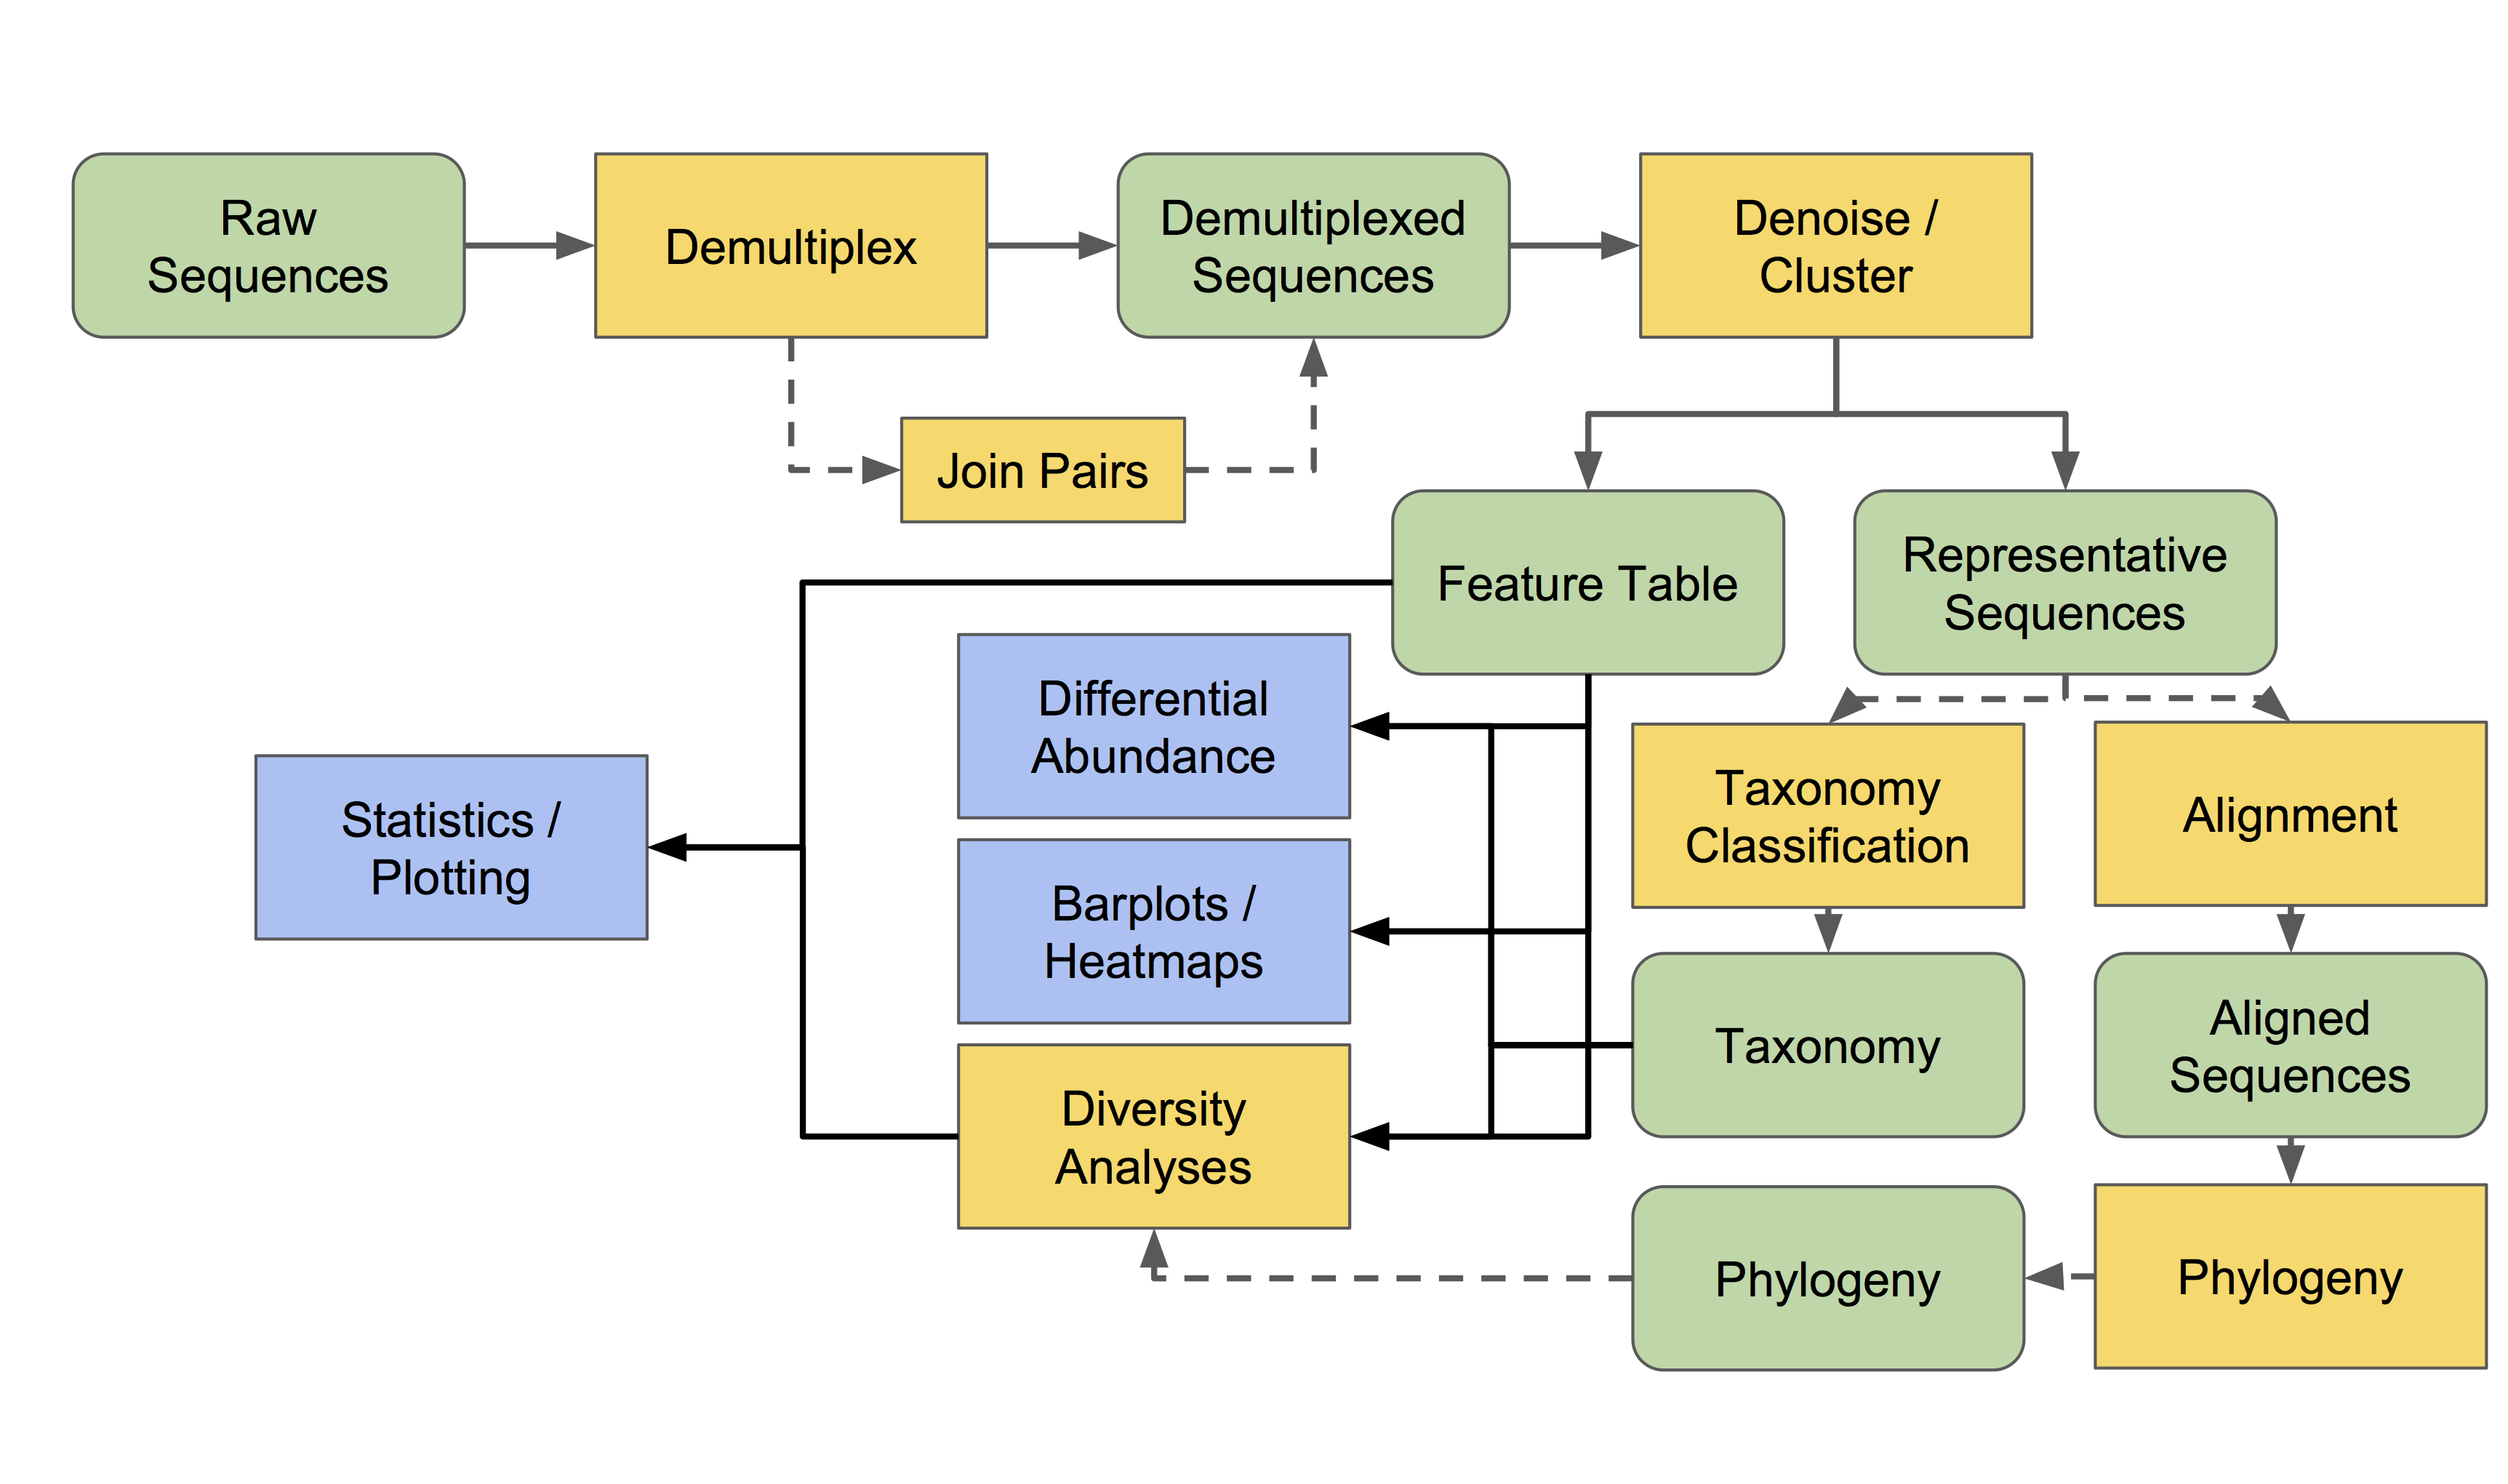
\includegraphics[width=0.8 \linewidth]{figures/qiime.png}
                \caption{A Theoretic Overview of QIIME2 Workflow \protect\cite{qiime1, qiime2}}
                \label{fig:qiime-workflow}
            \end{figure}

            \subsubsection{Denoising techniques}
                There are two denoising techniques provided by QIIME2: DADA2 \cite{DADA1} and Deblur \cite{deblur1}. Major difference between DADA2 and Deblur, as shown as figure \ref{fig:denosing-workflow}, is a strategy, the strategy used to divide as different species. DADA2 uses amplicon sequence variants (ASVs), strictly divides sequences even one-base mismatch. However, Deblur uses operational taxonomic units (OTUs), considers as same sequence when sequences are 97 \% or more matched.

                \begin{figure}[p]
                    \centering
                    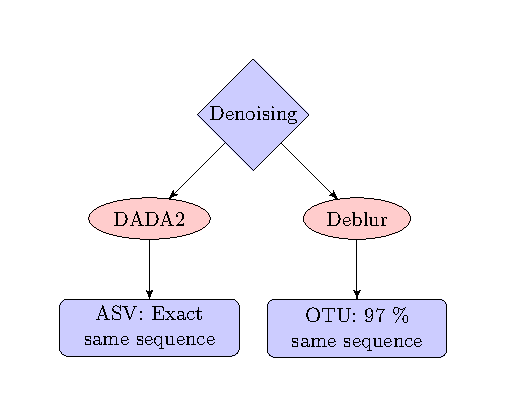
\includegraphics[width=0.5 \linewidth]{figures/denoising/denoising.pdf}
                    \caption{Denoising Techniques which provided by QIIME2}
                    \label{fig:denosing-workflow}
                \end{figure}

            \subsubsection{Taxonomy Classification}
                There are two taxonomy classification databases which provided by QIIME2: Greengenes (GG) \cite{greengenes1} and SILVA \cite{silva1}. Major difference between Greengenes and SILVA is resolution. Resolution of Greengenes is from kingdom to species; however, resolution of SILVA is from domain to genus. Note that a higher accuracy at taxonomic levels above genus level; but accuracy drops at species level \cite{performance1}.

                \begin{figure}[p]
                    \centering
                    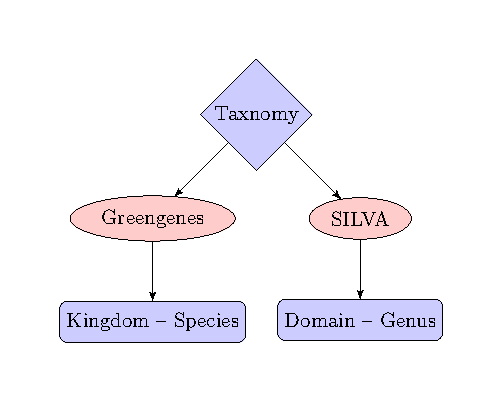
\includegraphics[width=0.5 \linewidth]{figures/taxonomy/taxonomy.pdf}
                    \caption{Taxonomy Classification which provided by QIIME2}
                    \label{fig:taxonomy-workflow}
                \end{figure}

            \subsubsection{Rarefaction}
                Rarefaction is a statistical method of estimating the number of species expected in a random sample which taken from a collection \cite{rarefaction1}. Moreover, rarefaction allows comparisons of the species richness among communities. Thus, rarefaction is a good choice for normalization \cite{rarefaction2}.

            \subsubsection{Alpha-diversity}
                Alpha-diversity is a metric which shows the richness of taxa at a single community. There are four alpha-diversity indices which provided from QIIME2:
                \begin{itemize}
                    \item Evenness index.
                    \item Faith's phylogenetic diversity.
                    \item Observed features.
                    \item Shannon's diversity index.
                \end{itemize}

                Shannon's diversity index shows a quantitative measure of community richness; Observed features, however, is a qualitative measure of community richness. Faith's phylogenetic diversity index indicates a qualitative measure of community richness which assimilates phylogenetic relationship among features. Finally, evenness index, as its name, shows a measure of community evenness.

            \subsubsection{Beta-diversity}
                Beta-diversity is a metric which indicates the taxonomic differentiation between multiple communities. There are four beta-diversity indices which provided from QIIME2:
                \begin{itemize}
                    \item Bray-Curtis distance.
                    \item Jaccard distance.
                    \item Unweighted UniFrac distance.
                    \item Weighted UniFrac distance.
                \end{itemize}

                Bray-Curtis distance shows a quantitative of community dissimilarity; Jaccard distance, however, indicates a qualitative measure of community dissimilarity. UniFrac distances reveal a measure of community dissimilarity which consolidates phylogenetic relationship among features. Difference between unweighted UniFrac distance and weighted UniFrac distance is a qualitative and a quantitative, respectively.

            \subsubsection{ANCOM}
                ANCOM (Analysis of composition of microbiomes) can be used for analyzing the composition of microbiome in multiple populations \cite{ANCOM1}. Example ANCOM volcano plot is shows as figure \ref{fig:ancom-example}.

                \begin{figure}[p]
                    \centering
                    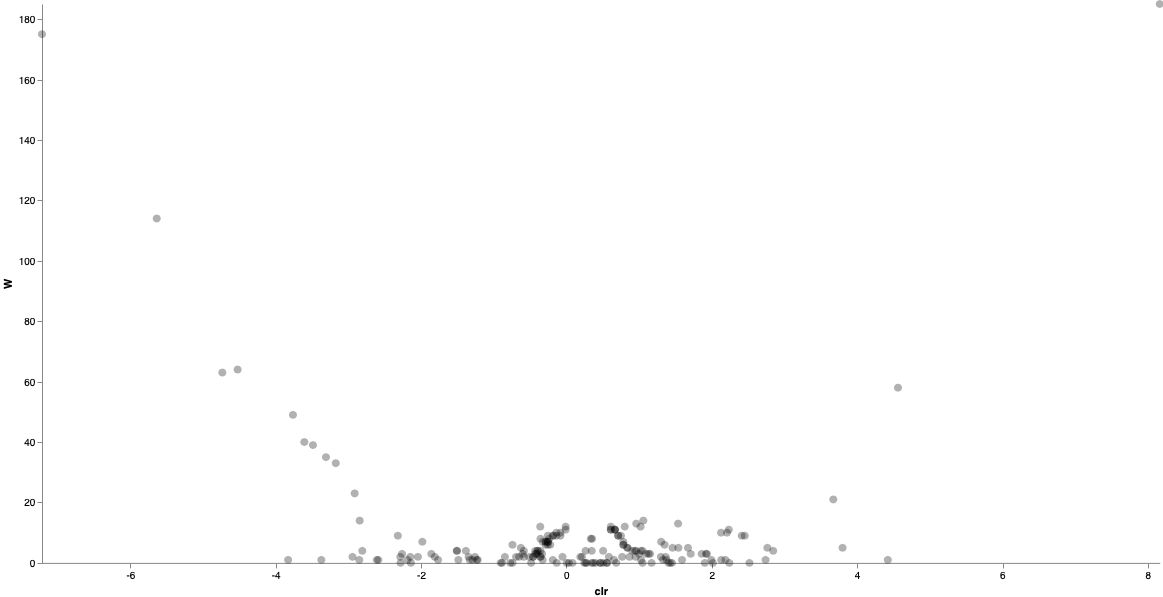
\includegraphics[width=0.8 \linewidth]{figures/ANCOM/example.png}
                    \caption{Example ANCOM Volcano Plot which Provided by QIIME2 \protect\cite{qiime1, qiime2}}
                    \label{fig:ancom-example}
                \end{figure}

        \subsection{Python Packages}
            \subsubsection{Pandas}
                Pandas is a Python package of rich data structures and tools for analyzing with structured data sets \cite{pandas1}.

            \subsubsection{Scikit-learn}
                Scikit-learn grants state-of-the-art implementation of many machine learning algorithms, while controlling an easy-to-use interface tightly integrated the Python code \cite{sklearn1}.

            \subsubsection{Matplotlib}
                Matplotlib is a Python graphics package which used for application development, interactive scripting and publication quality image generation \cite{matplotlib2}. Matplotlib, also, is designed to create simple plots with a few commands \cite{matplotlib1}.

            \subsubsection{Seaborn}
                Seaborn is a Python data visualization package which based on matplotlib, allows a high-level interface for displaying engaging and descriptive statistical graphics \cite{seaborn1}.

    \section{Results}
        \subsection{Quality Filter}
            Longer sequences have more fallen sequence quality than shorter. Thus, sequences which longer than threshold should be trimmed out due to their low quality. However, gold-standard strategy for deciding the threshold does not exist; the threshold is set as longest sequence length which have half of sequences have greater than 30 quality score. Hence, sequence quality plot is shown as figure \ref{fig:sequence-quality}; trimmed length in forward reads is 300, and trimmed length in reverse reads is 265.

            \begin{figure}[p]
                \centering
                $\begin{array}{cc}
                    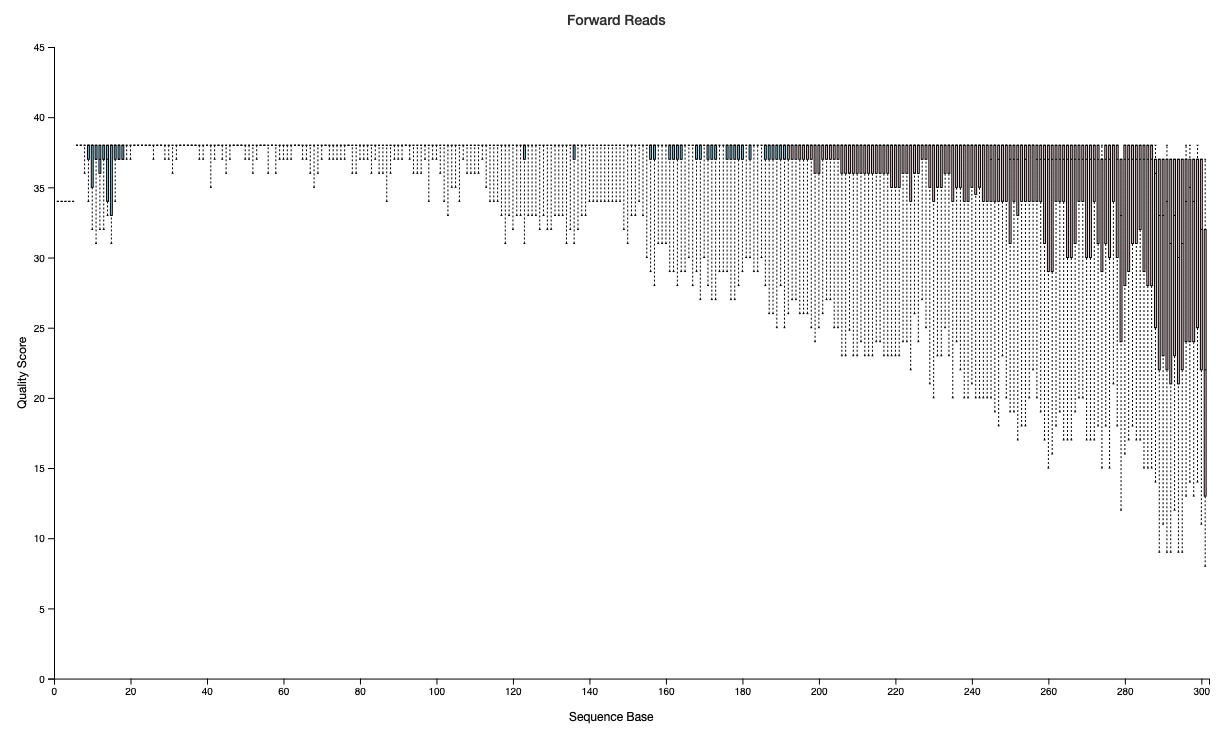
\includegraphics[width=0.4 \linewidth]{figures/QualityFilter/Forward.png}
                    &
                    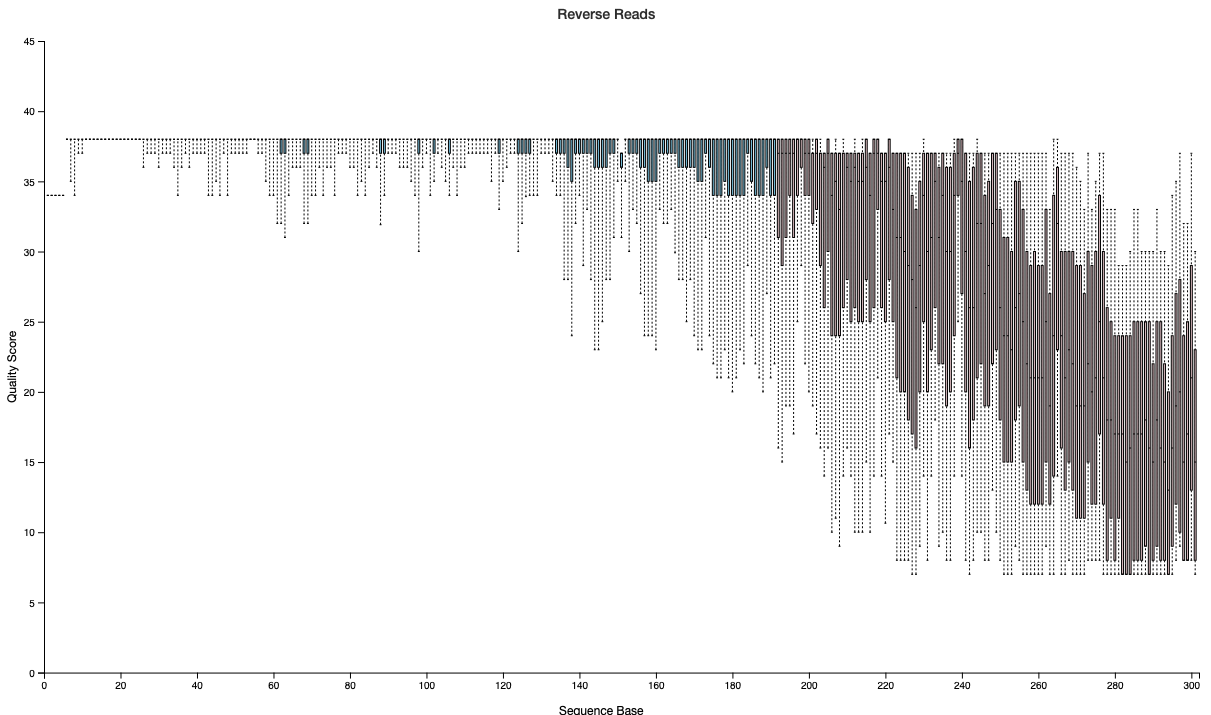
\includegraphics[width=0.4 \linewidth]{figures/QualityFilter/Reverse.png}
                    \\
                    \mbox{(a) Forward Reads} & \mbox{(b) Reverse Reads} \\
                \end{array}$
                \caption{Sequence Quality Plot}
                \label{fig:sequence-quality}
            \end{figure}

        \subsection{Rarefaction}
            Sampling depth should be decided for rarefaction. Gold-standard method for determining sampling depth is minimum frequency in the samples. Hence, sampling depth with DADA2 is 3786 (Figure \ref{fig:frequency-sample-dada2}), and sampling depth with Deblur is 7253 (Figure \ref{fig:frequency-sample-deblur}).

            \begin{figure}[p]
                \centering
                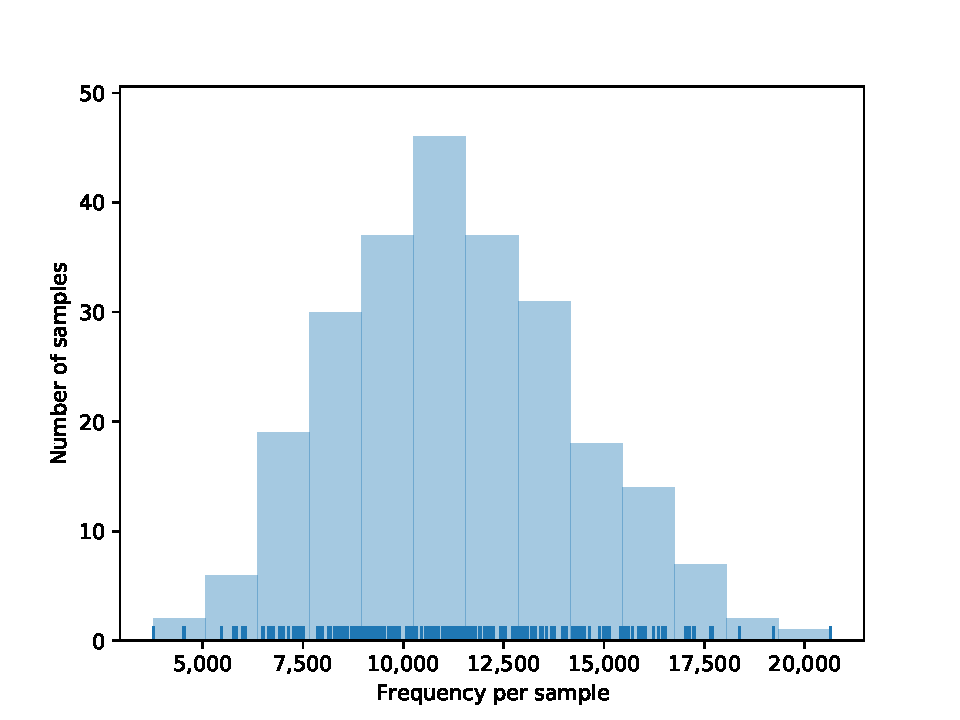
\includegraphics[width=0.6 \linewidth]{figures/Rarefaction/DADA.pdf}
                \caption{Frequency per Sample by DADA2}
                \label{fig:frequency-sample-dada2}
            \end{figure}

            \begin{figure}[p]
                \centering
                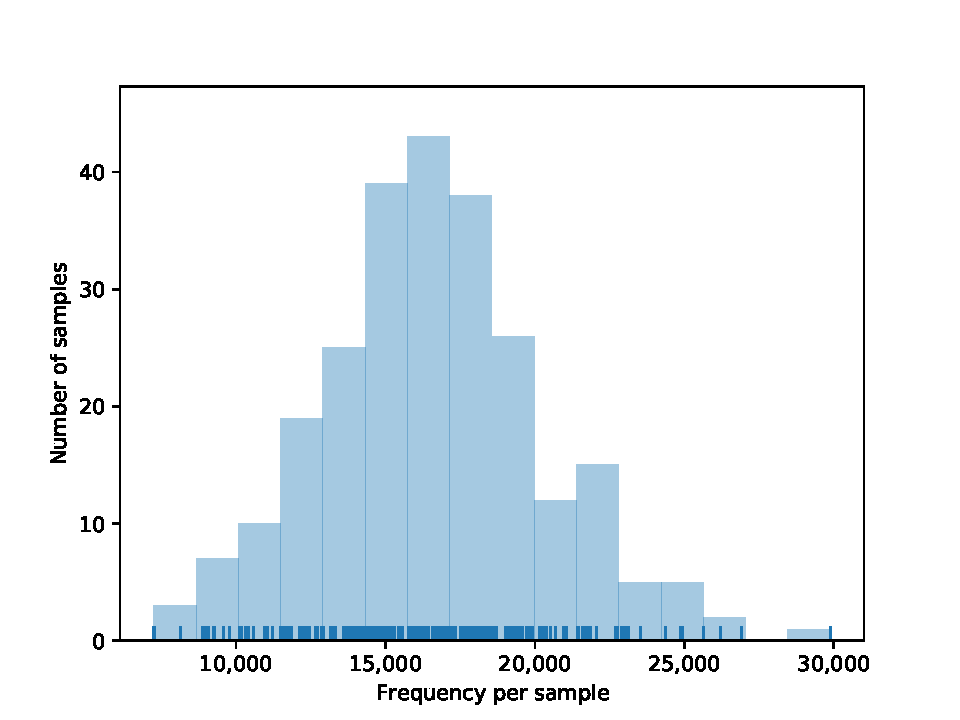
\includegraphics[width=0.6 \linewidth]{figures/Rarefaction/Deblur.pdf}
                \caption{Frequency per Sample by DADA2}
                \label{fig:frequency-sample-deblur}
            \end{figure}

        \subsection{Alpha-diversity}

            \begin{table}[p]
                \centering
                \caption{Kruskal-Wallis among All Group with DADA2}
                \label{tb:alpha-all-dada2}
                \csvautobooktabular{csv/AlphaDiversity/DADA2/all.csv}
            \end{table}

            \begin{table}[p]
                \centering
                \caption{Kruskal-Wallis from Evenness Index with DADA2}
                \label{tb:alpha-evenness-dada2}
                \csvautobooktabular{csv/AlphaDiversity/DADA2/evenness.csv}
            \end{table}

            \begin{table}[p]
                \centering
                \caption{Kruskal-Wallis from Faith PD Index with DADA2}
                \label{tb:alpha-faith-dada2}
                \csvautobooktabular{csv/AlphaDiversity/DADA2/faith.csv}
            \end{table}

            \begin{table}[p]
                \centering
                \caption{Kruskal-Wallis from Observed Features Index with DADA2}
                \label{tb:alpha-observed-dada2}
                \csvautobooktabular{csv/AlphaDiversity/DADA2/observed.csv}
            \end{table}

            \begin{table}[p]
                \centering
                \caption{Kruskal-Wallis from Shannon's Diversity Index with DADA2}
                \label{tb:alpha-shannon-dada2}
                \csvautobooktabular{csv/AlphaDiversity/DADA2/shannon.csv}
            \end{table}

            \begin{figure}[p]
                \centering
                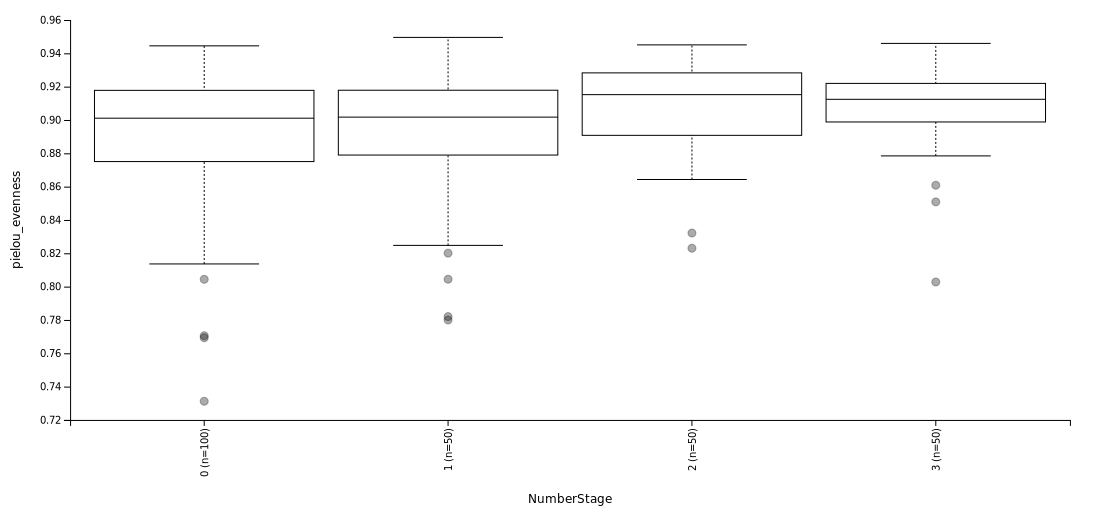
\includegraphics[width=0.8 \linewidth]{figures/AlphaDiversity/DADA2/evenness.png}
                \caption{Evenness Index from DADA2}
                \label{fig:evenness-dada2}
            \end{figure}

            \begin{figure}[p]
                \centering
                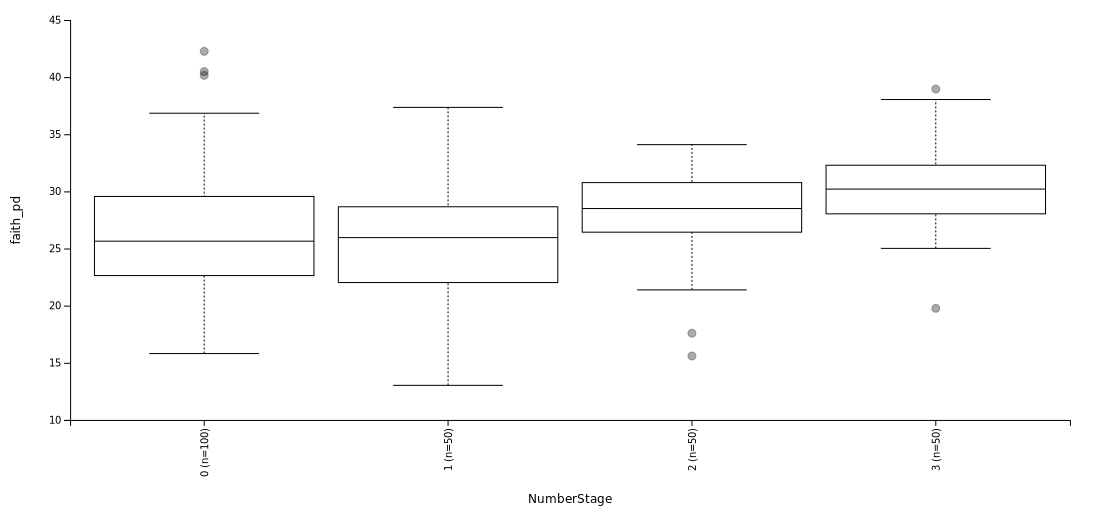
\includegraphics[width=0.8 \linewidth]{figures/AlphaDiversity/DADA2/faith.png}
                \caption{Faith PD Index from DADA2}
                \label{fig:faith-dada2}
            \end{figure}

            \begin{figure}[p]
                \centering
                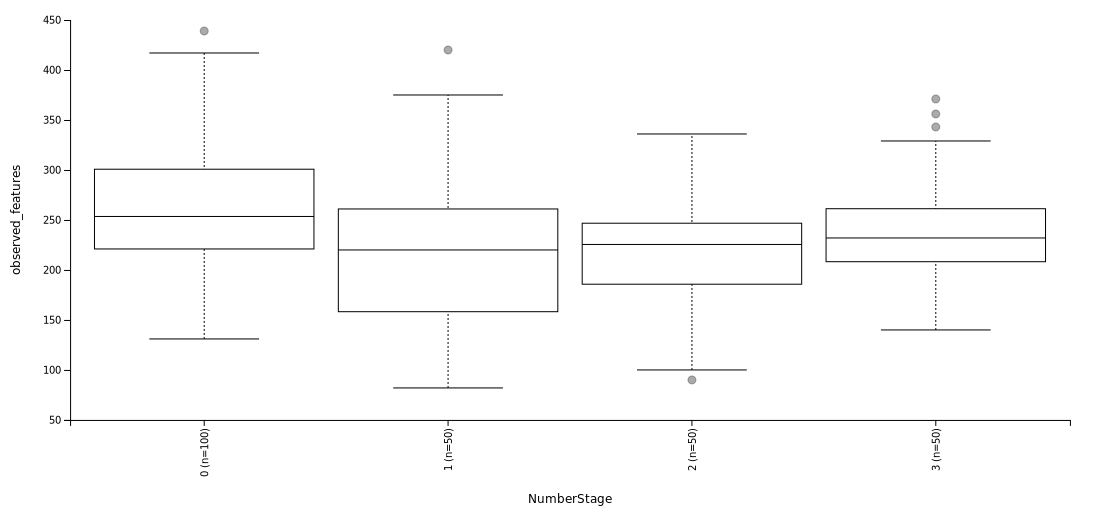
\includegraphics[width=0.8 \linewidth]{figures/AlphaDiversity/DADA2/observed.png}
                \caption{Observed Features Index from DADA2}
                \label{fig:observed-dada2}
            \end{figure}

            \begin{figure}[p]
                \centering
                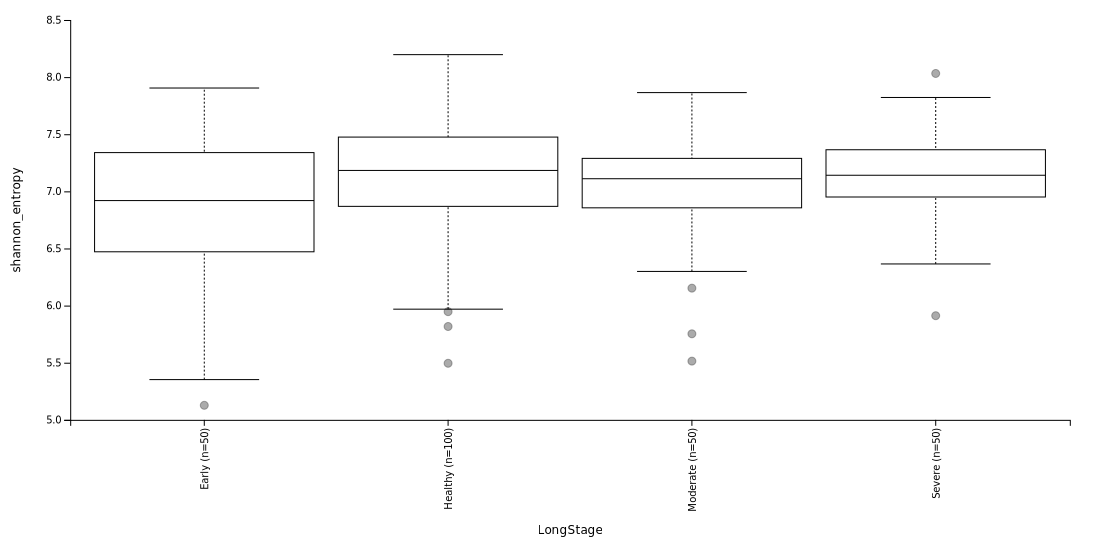
\includegraphics[width=0.8 \linewidth]{figures/AlphaDiversity/DADA2/shannon.png}
                \caption{Shannon's Diversity Index from DADA2}
                \label{fig:shannon-dada2}
            \end{figure}

            \begin{table}[p]
                \centering
                \caption{Kruskal-Wallis among All Group with Deblur}
                \label{tb:alpha-all-deblur}
                \csvautobooktabular{csv/AlphaDiversity/Deblur/all.csv}
            \end{table}

            \begin{table}[p]
                \centering
                \caption{Kruskal-Wallis from Evenness Index with Deblur}
                \label{tb:alpha-evenness-deblur}
                \csvautobooktabular{csv/AlphaDiversity/Deblur/evenness.csv}
            \end{table}

            \begin{table}[p]
                \centering
                \caption{Kruskal-Wallis from Faith PD Index with Deblur}
                \label{tb:alpha-faith-deblur}
                \csvautobooktabular{csv/AlphaDiversity/Deblur/faith.csv}
            \end{table}

            \begin{table}[p]
                \centering
                \caption{Kruskal-Wallis from Observed Features Index with Deblur}
                \label{tb:alpha-observed-deblur}
                \csvautobooktabular{csv/AlphaDiversity/Deblur/observed.csv}
            \end{table}

            \begin{table}[p]
                \centering
                \caption{Kruskal-Wallis from Shannon's Diversity Index with Deblur}
                \label{tb:alpha-shannon-deblur}
                \csvautobooktabular{csv/AlphaDiversity/Deblur/shannon.csv}
            \end{table}

            \begin{figure}[p]
                \centering
                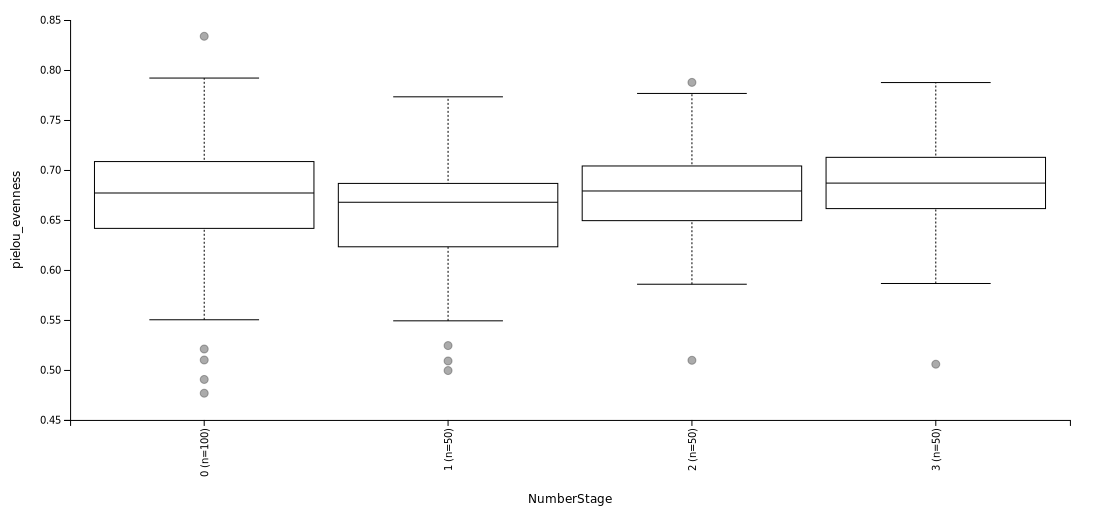
\includegraphics[width=0.8 \linewidth]{figures/AlphaDiversity/Deblur/evenness.png}
                \caption{Evenness Index from Deblur}
                \label{fig:evenness-deblur}
            \end{figure}

            \begin{figure}[p]
                \centering
                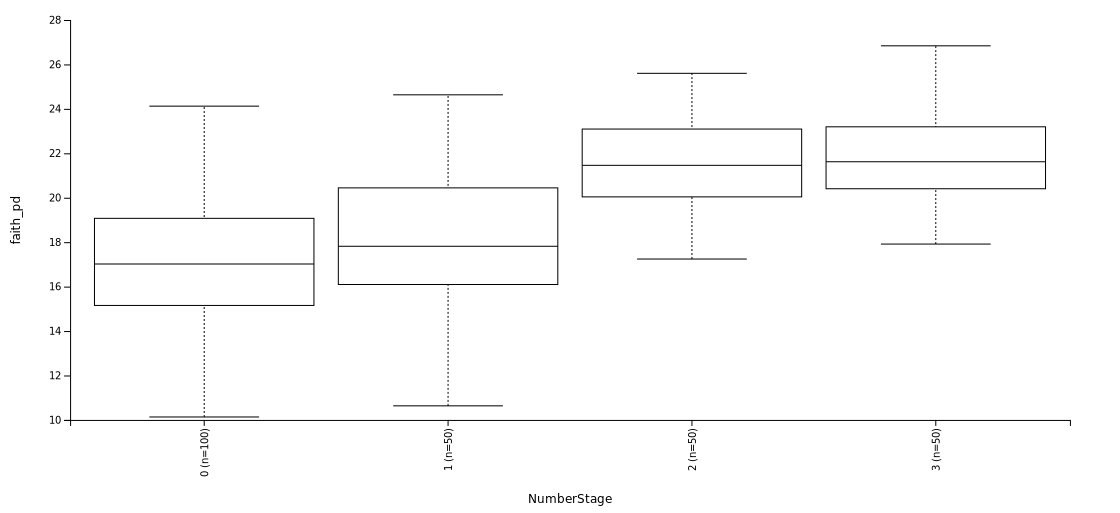
\includegraphics[width=0.8 \linewidth]{figures/AlphaDiversity/Deblur/faith.png}
                \caption{Faith PD Index from Deblur}
                \label{fig:faith-deblur}
            \end{figure}

            \begin{figure}[p]
                \centering
                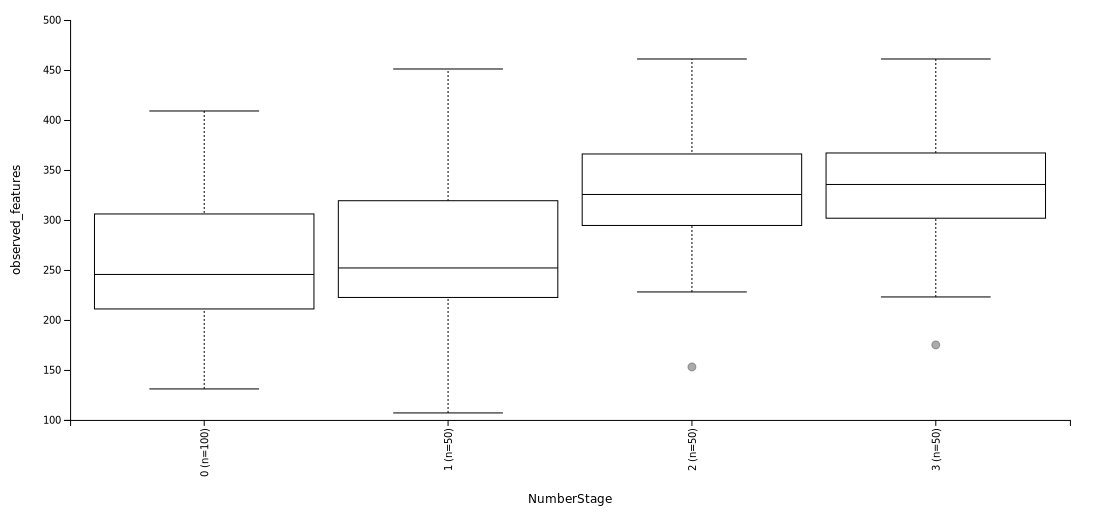
\includegraphics[width=0.8 \linewidth]{figures/AlphaDiversity/Deblur/observed.png}
                \caption{Observed Features Index from Deblur}
                \label{fig:observed-deblur}
            \end{figure}

            \begin{figure}[p]
                \centering
                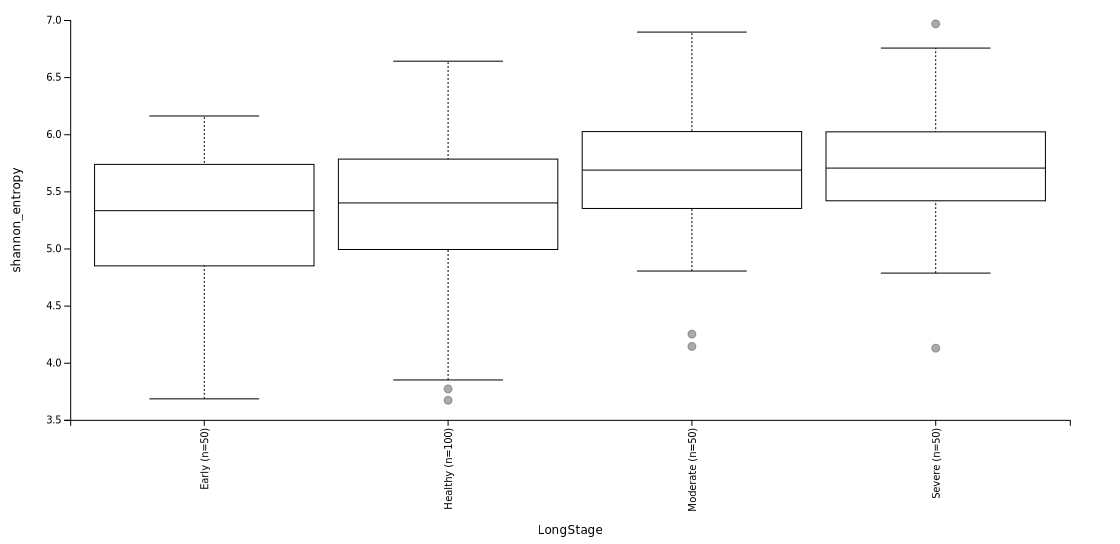
\includegraphics[width=0.8 \linewidth]{figures/AlphaDiversity/Deblur/shannon.png}
                \caption{Shannon's Diversity Index from Deblur}
                \label{fig:shannon-deblur}
            \end{figure}

        \subsection{Beta-diversity}

            \begin{table}[p]
                \centering
                \caption{Bray-Curtis Distance Index with DADA2}
                \label{tb:bray-dada2}
                \csvautobooktabular{csv/BetaDiversity/DADA2/Bray.csv}
            \end{table}

            \begin{table}[p]
                \centering
                \caption{Jaccard Distance Index with DADA2}
                \label{tb:jaccard-dada2}
                \csvautobooktabular{csv/BetaDiversity/DADA2/Jaccard.csv}
            \end{table}

            \begin{table}[p]
                \centering
                \caption{Unweighted UniFrac Distance Index with DADA2}
                \label{tb:unweighted-dada2}
                \csvautobooktabular{csv/BetaDiversity/DADA2/UnweightedUniFrac.csv}
            \end{table}

            \begin{table}[p]
                \centering
                \caption{Weighted UniFrac Distance Index with DADA2}
                \label{tb:weighted-dada2}
                \csvautobooktabular{csv/BetaDiversity/DADA2/WeightedUniFrac.csv}
            \end{table}

            \begin{figure}[p]
                \centering
                $\begin{array}{cc}
                    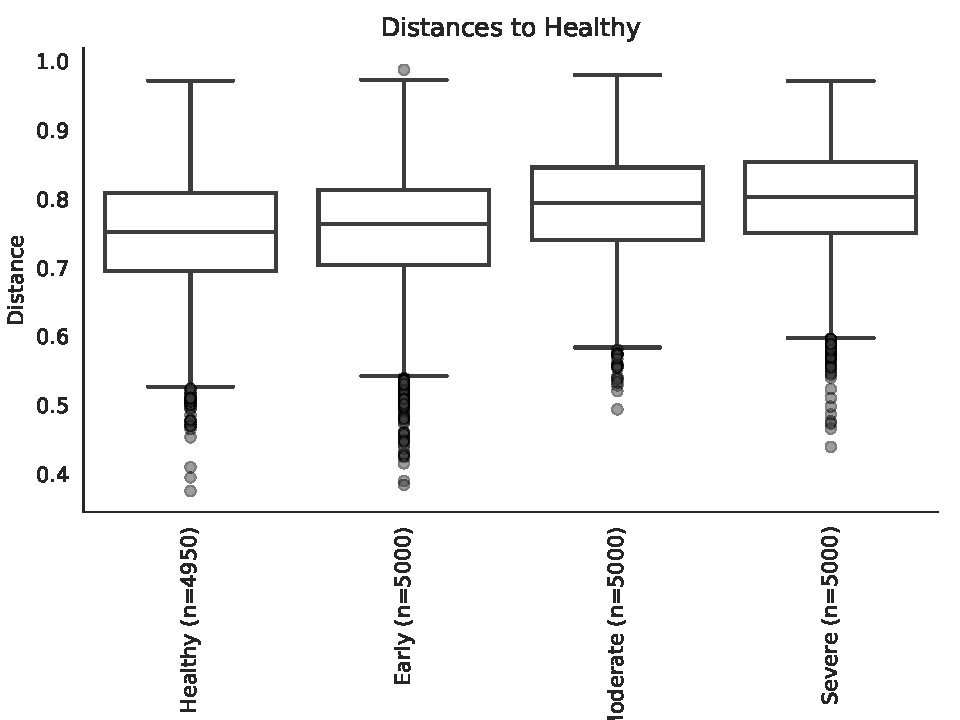
\includegraphics[width=0.4 \linewidth]{figures/BetaDiversity/DADA2/Bray/Healthy.pdf}
                    &
                    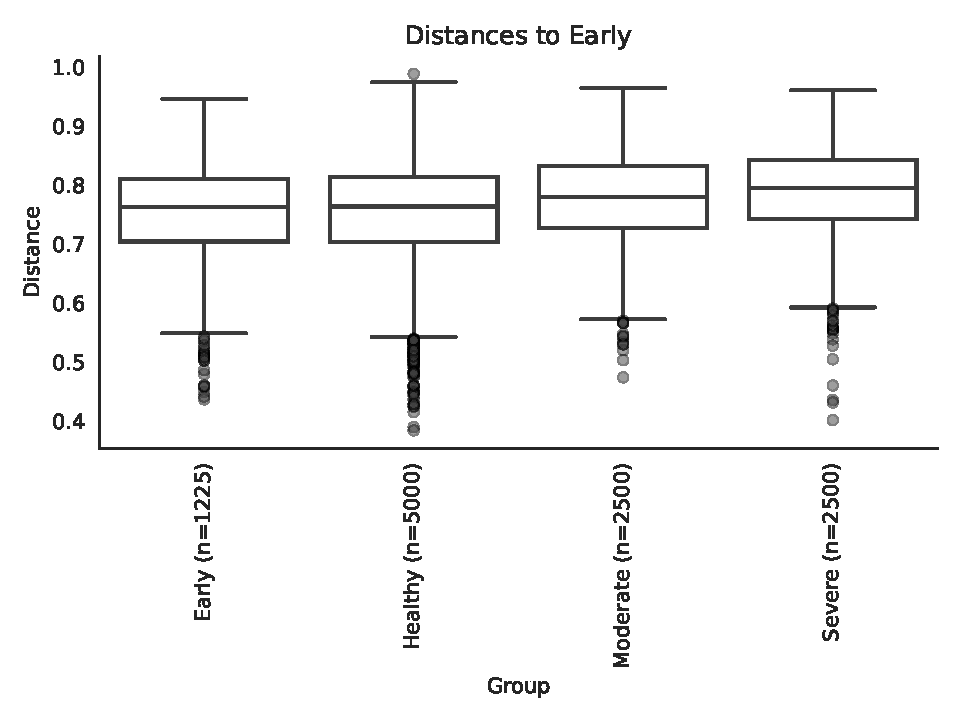
\includegraphics[width=0.4 \linewidth]{figures/BetaDiversity/DADA2/Bray/Early.pdf}
                    \\
                    \mbox{(a) Healthy} & \mbox{(b) Early} \\

                    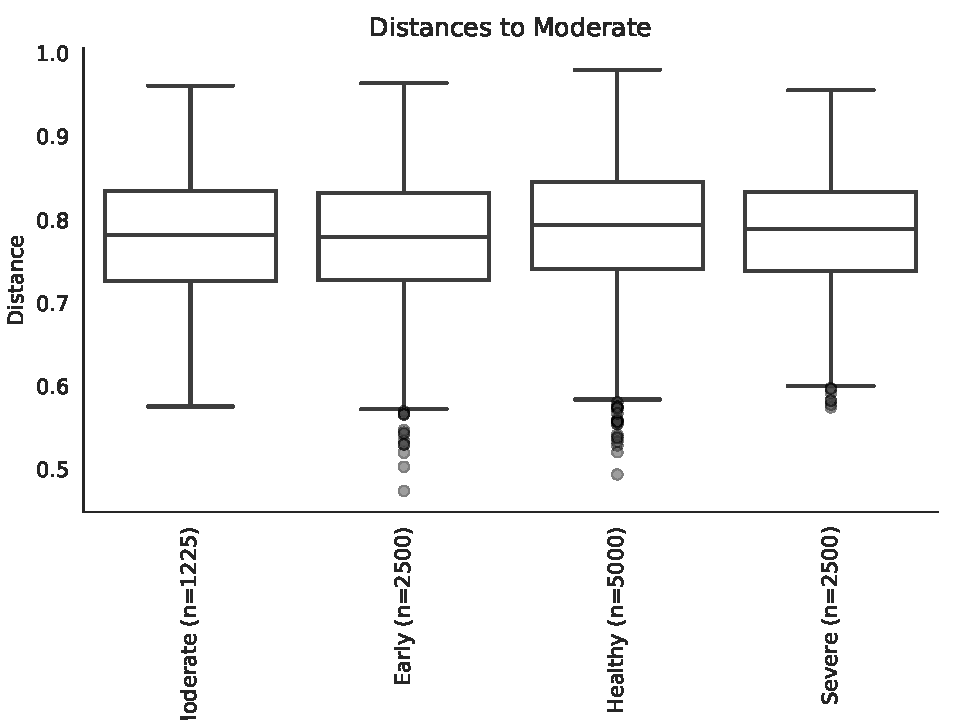
\includegraphics[width=0.4 \linewidth]{figures/BetaDiversity/DADA2/Bray/Moderate.pdf}
                    &
                    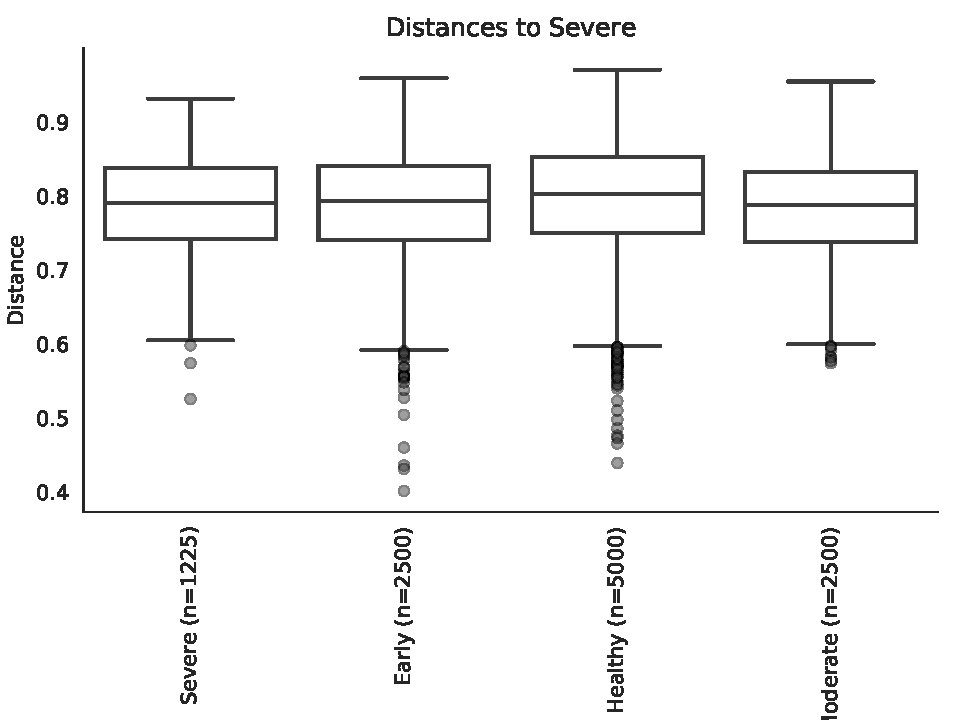
\includegraphics[width=0.4 \linewidth]{figures/BetaDiversity/DADA2/Bray/Severe.pdf}
                    \\
                    \mbox{(c) Moderate} & \mbox{(d) Severe} \\
                \end{array}$
                \caption{Bray-Curtis Distance Index with DADA2}
                \label{fig:bray-dada2}
            \end{figure}

            \begin{figure}[p]
                \centering
                $\begin{array}{cc}
                    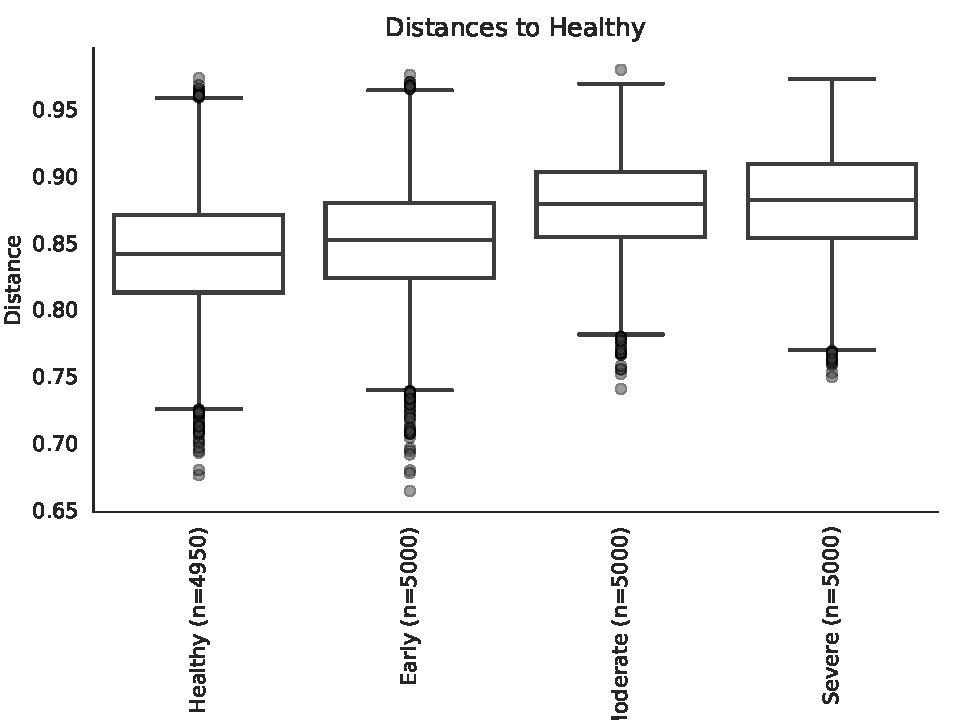
\includegraphics[width=0.4 \linewidth]{figures/BetaDiversity/DADA2/Jaccard/Healthy.pdf}
                    &
                    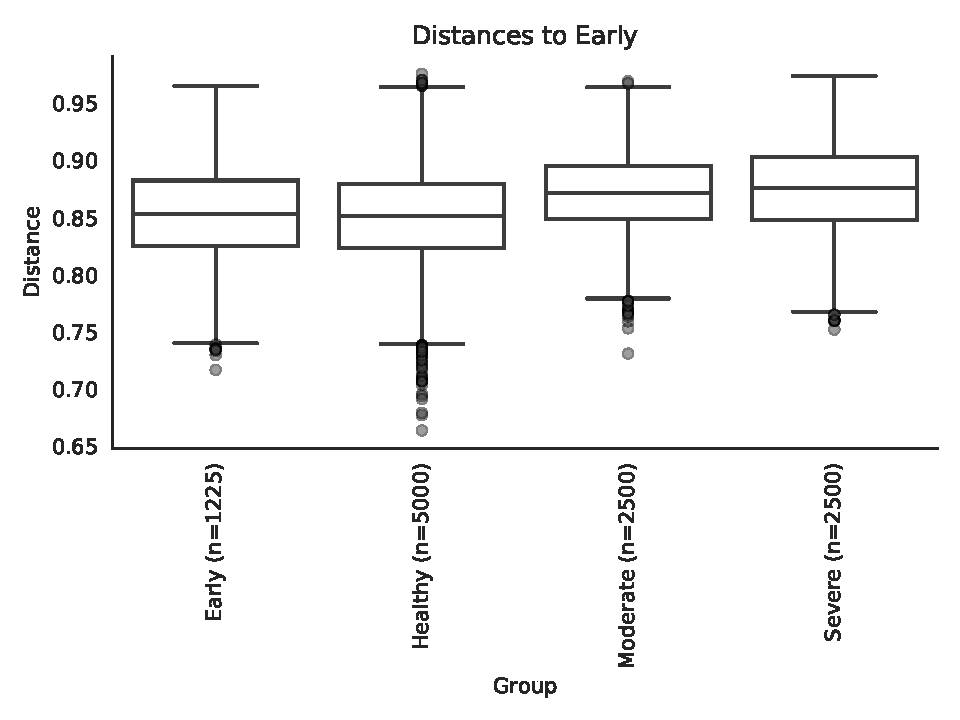
\includegraphics[width=0.4 \linewidth]{figures/BetaDiversity/DADA2/Jaccard/Early.pdf}
                    \\
                    \mbox{(a) Healthy} & \mbox{(b) Early} \\

                    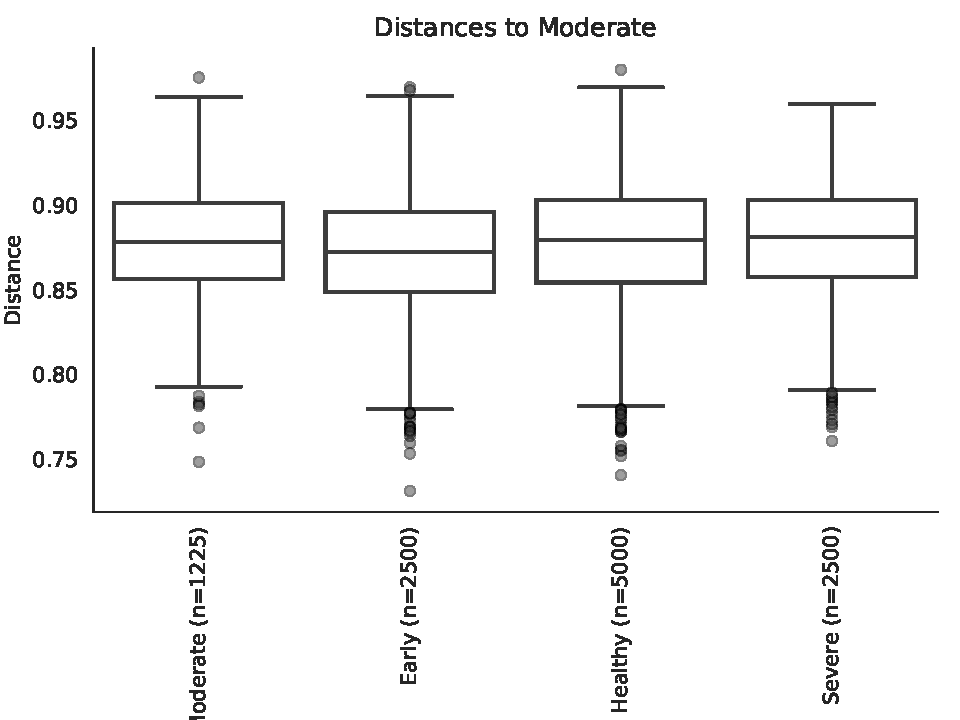
\includegraphics[width=0.4 \linewidth]{figures/BetaDiversity/DADA2/Jaccard/Moderate.pdf}
                    &
                    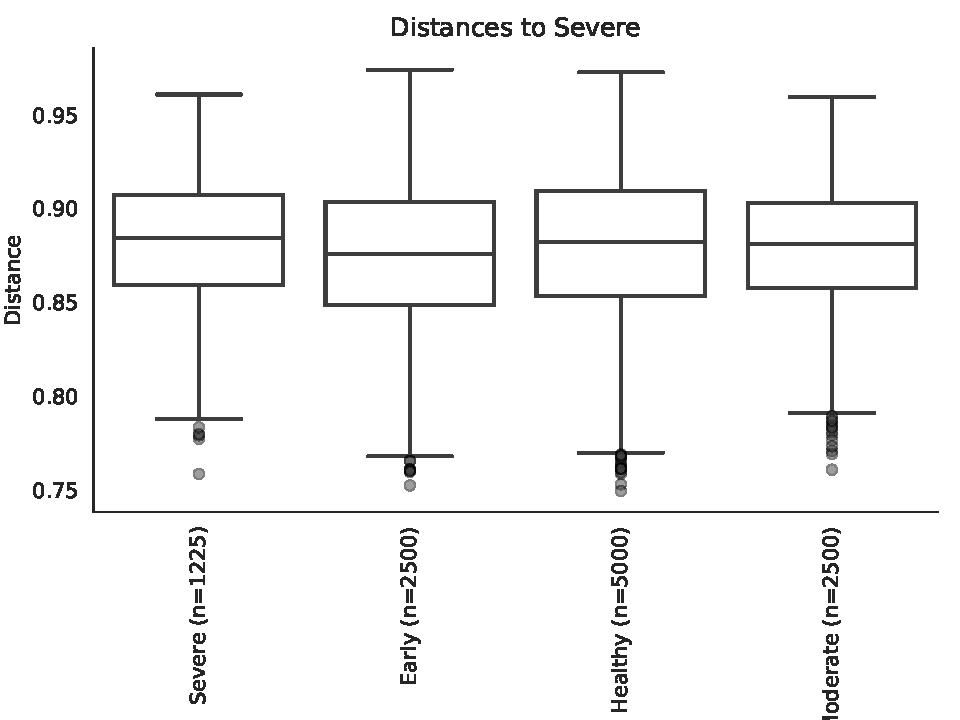
\includegraphics[width=0.4 \linewidth]{figures/BetaDiversity/DADA2/Jaccard/Severe.pdf}
                    \\
                    \mbox{(c) Moderate} & \mbox{(d) Severe} \\
                \end{array}$
                \caption{Jaccard Distance Index with DADA2}
                \label{fig:jaccard-dada2}
            \end{figure}

            \begin{figure}[p]
                \centering
                $\begin{array}{cc}
                    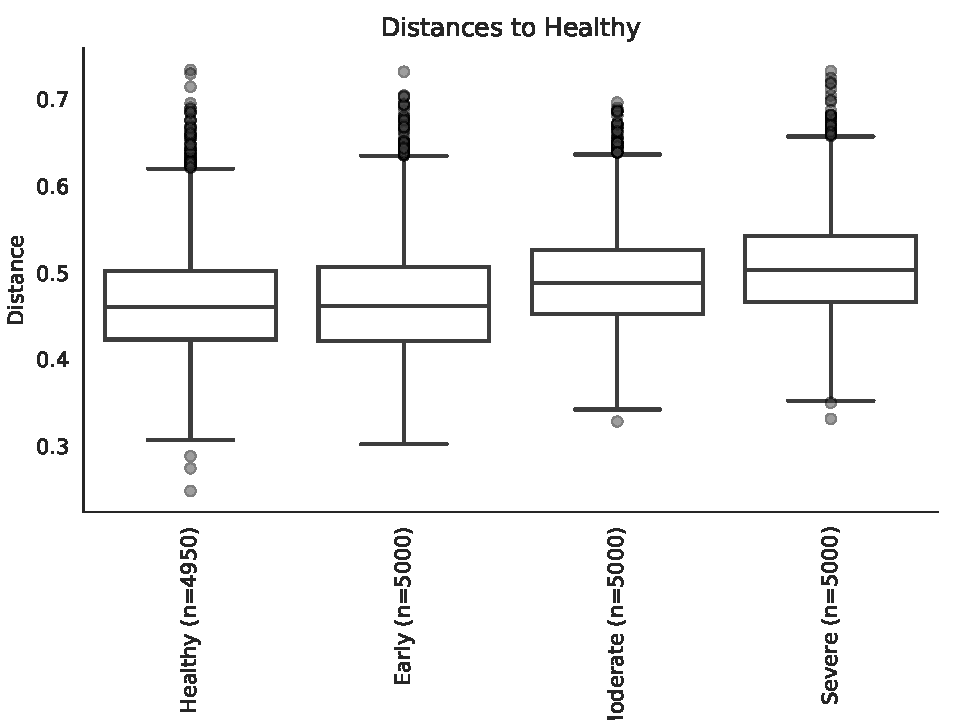
\includegraphics[width=0.4 \linewidth]{figures/BetaDiversity/DADA2/UnweightedUnifrac/Healthy.pdf}
                    &
                    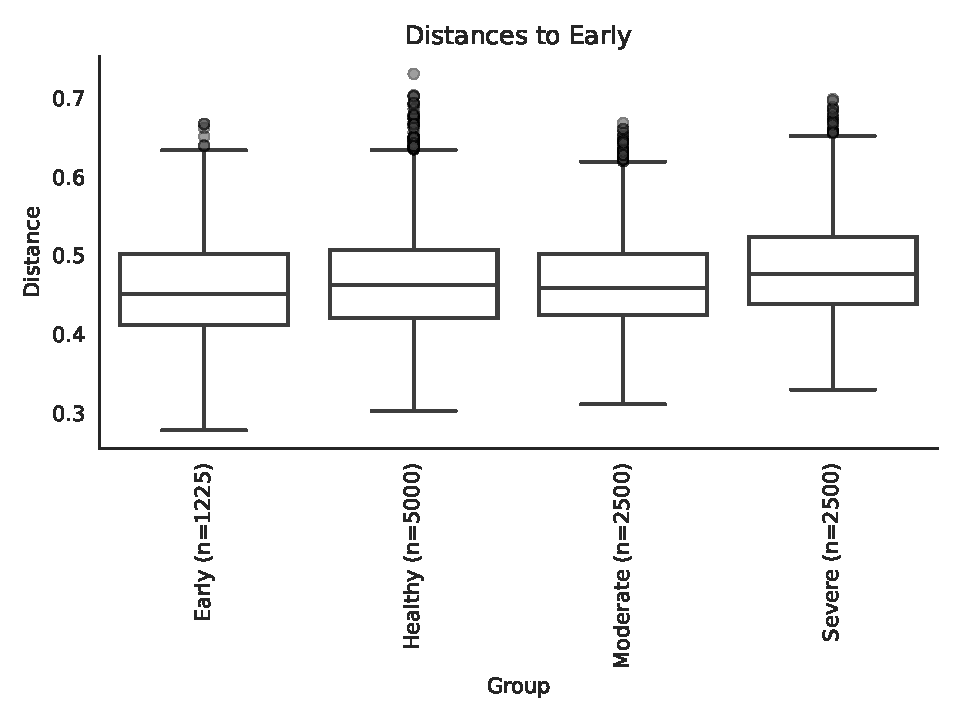
\includegraphics[width=0.4 \linewidth]{figures/BetaDiversity/DADA2/UnweightedUnifrac/Early.pdf}
                    \\
                    \mbox{(a) Healthy} & \mbox{(b) Early} \\

                    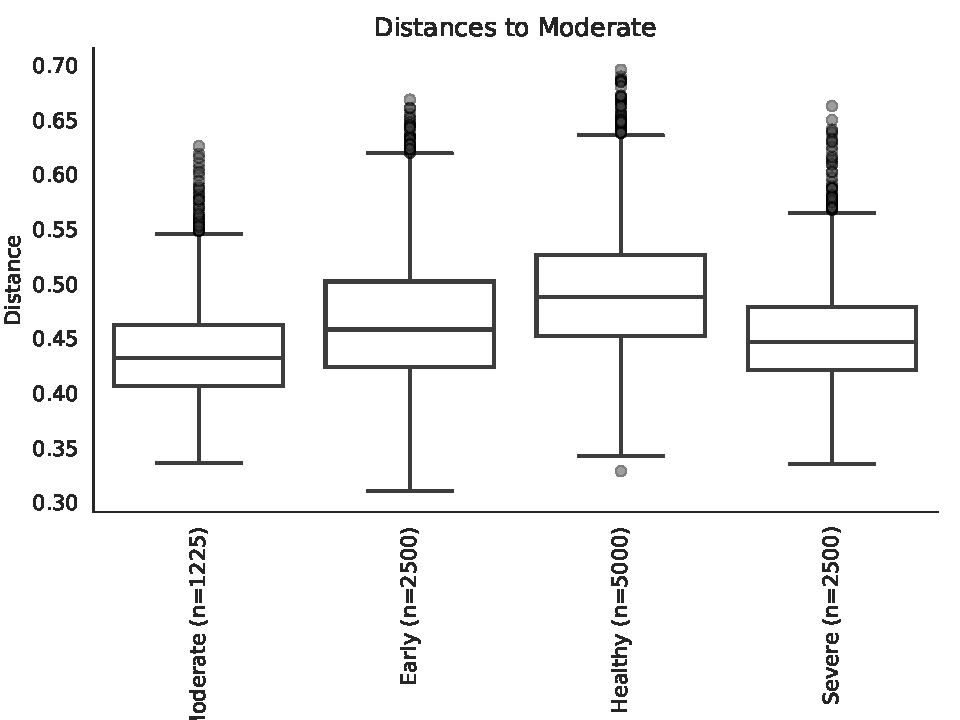
\includegraphics[width=0.4 \linewidth]{figures/BetaDiversity/DADA2/UnweightedUnifrac/Moderate.pdf}
                    &
                    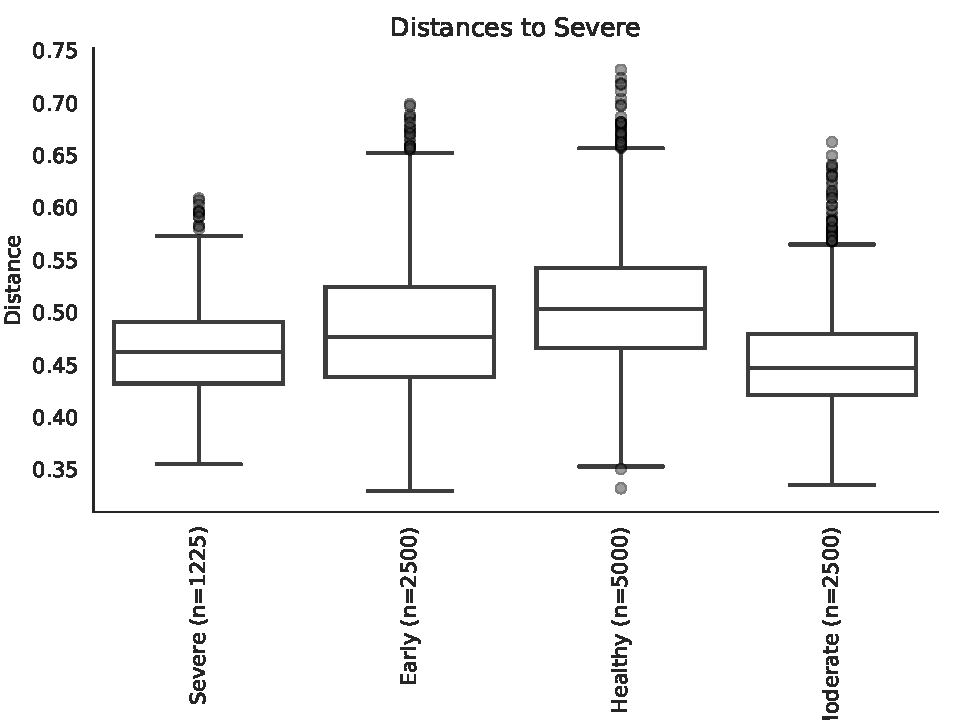
\includegraphics[width=0.4 \linewidth]{figures/BetaDiversity/DADA2/UnweightedUnifrac/Severe.pdf}
                    \\
                    \mbox{(c) Moderate} & \mbox{(d) Severe} \\
                \end{array}$
                \caption{Unweighted Unifrac Distance Index with DADA2}
                \label{fig:unweighted-dada2}
            \end{figure}

            \begin{figure}[p]
                \centering
                $\begin{array}{cc}
                    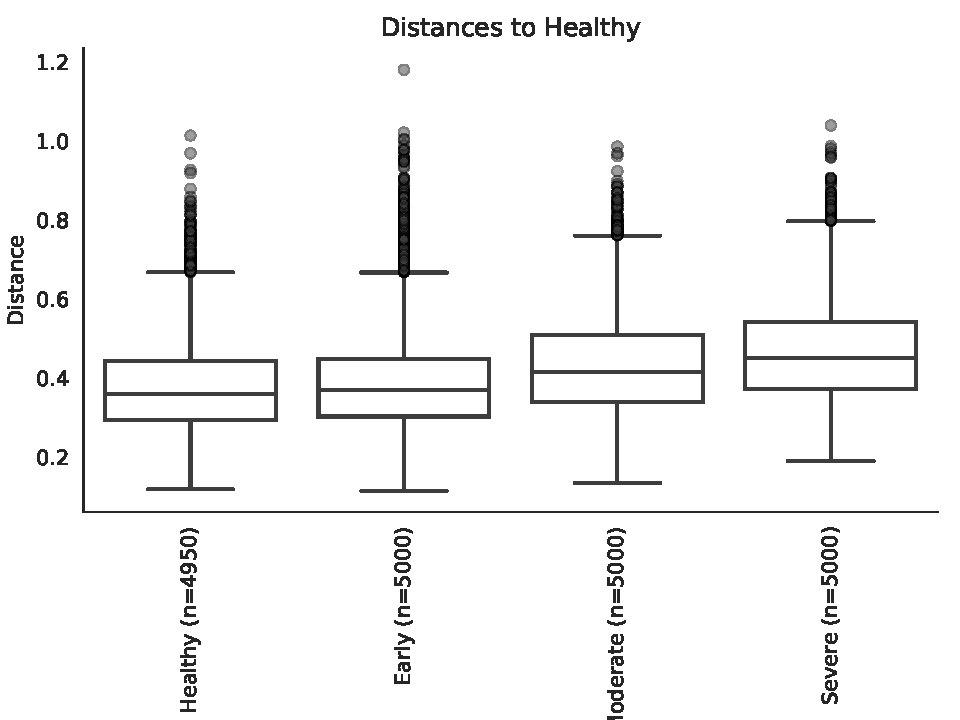
\includegraphics[width=0.4 \linewidth]{figures/BetaDiversity/DADA2/WeightedUnifrac/Healthy.pdf}
                    &
                    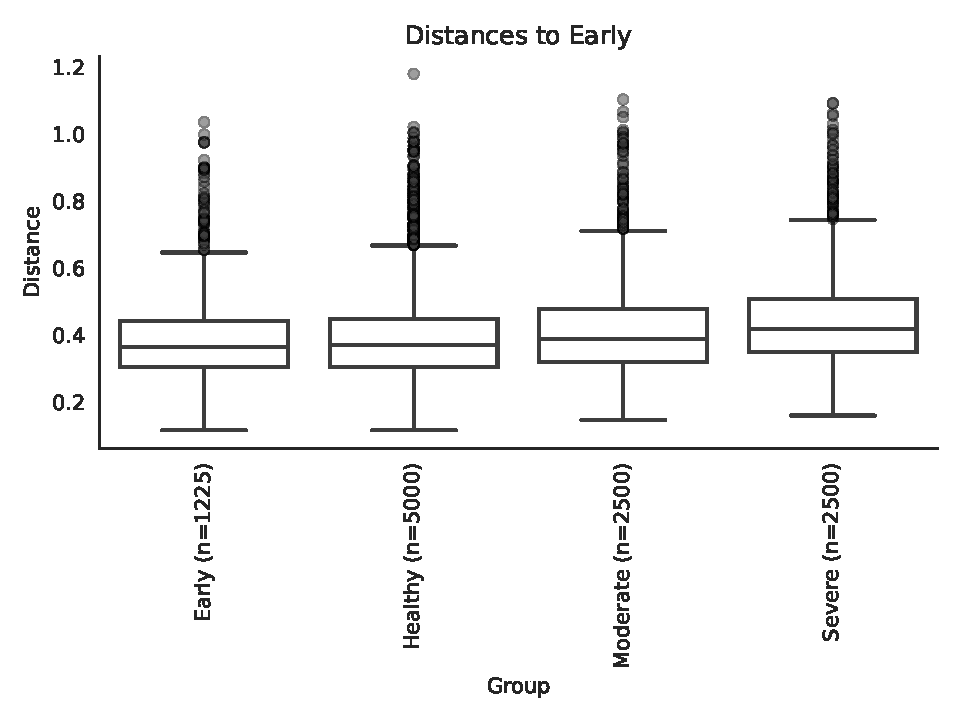
\includegraphics[width=0.4 \linewidth]{figures/BetaDiversity/DADA2/WeightedUnifrac/Early.pdf}
                    \\
                    \mbox{(a) Healthy} & \mbox{(b) Early} \\

                    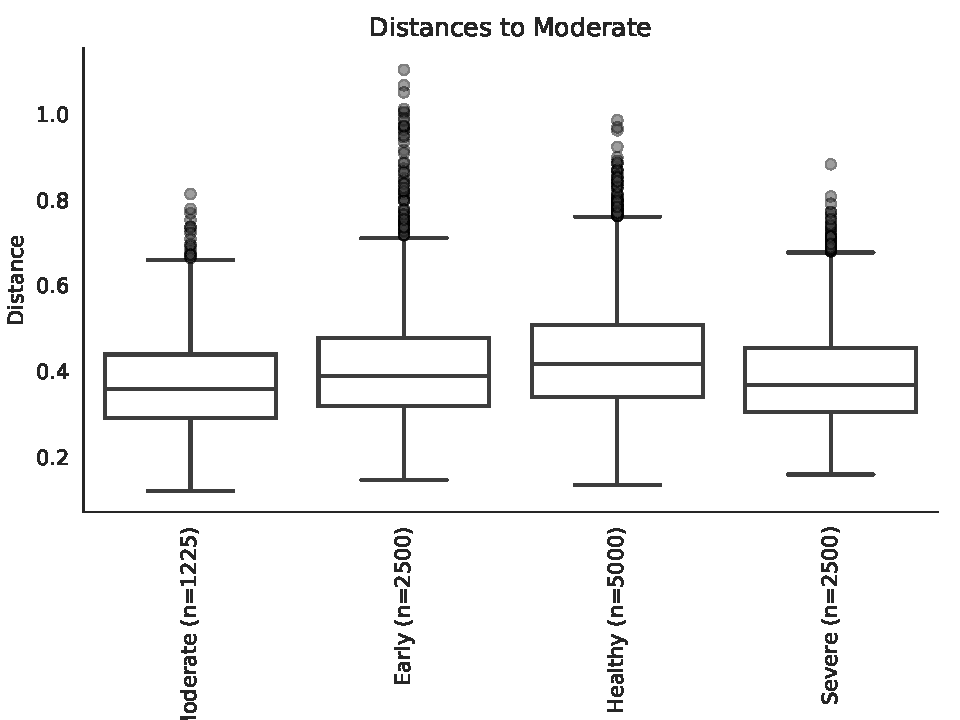
\includegraphics[width=0.4 \linewidth]{figures/BetaDiversity/DADA2/WeightedUnifrac/Moderate.pdf}
                    &
                    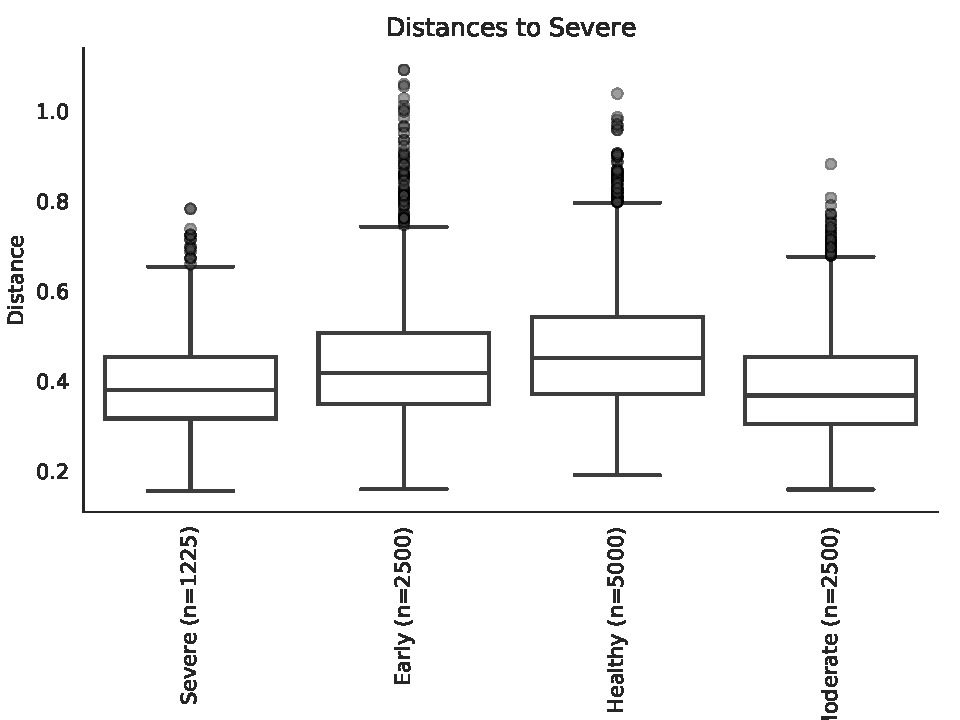
\includegraphics[width=0.4 \linewidth]{figures/BetaDiversity/DADA2/WeightedUnifrac/Severe.pdf}
                    \\
                    \mbox{(c) Moderate} & \mbox{(d) Severe} \\
                \end{array}$
                \caption{Weighted Unifrac Distance Index with DADA2}
                \label{fig:weighted-dada2}
            \end{figure}

            \begin{table}[p]
                \centering
                \caption{Bray-Curtis Distance Index with Deblur}
                \label{tb:bray-deblur}
                \csvautobooktabular{csv/BetaDiversity/Deblur/Bray.csv}
            \end{table}

            \begin{table}[p]
                \centering
                \caption{Jaccard Distance Index with Deblur}
                \label{tb:jaccard-deblur}
                \csvautobooktabular{csv/BetaDiversity/Deblur/Jaccard.csv}
            \end{table}

            \begin{table}[p]
                \centering
                \caption{Unweighted UniFrac Distance Index with Deblur}
                \label{tb:unweighted-deblur}
                \csvautobooktabular{csv/BetaDiversity/Deblur/UnweightedUniFrac.csv}
            \end{table}

            \begin{table}[p]
                \centering
                \caption{Weighted UniFrac Distance Index with Deblur}
                \label{tb:weighted-deblur}
                \csvautobooktabular{csv/BetaDiversity/Deblur/WeightedUniFrac.csv}
            \end{table}

            \begin{figure}[p]
                \centering
                $\begin{array}{cc}
                    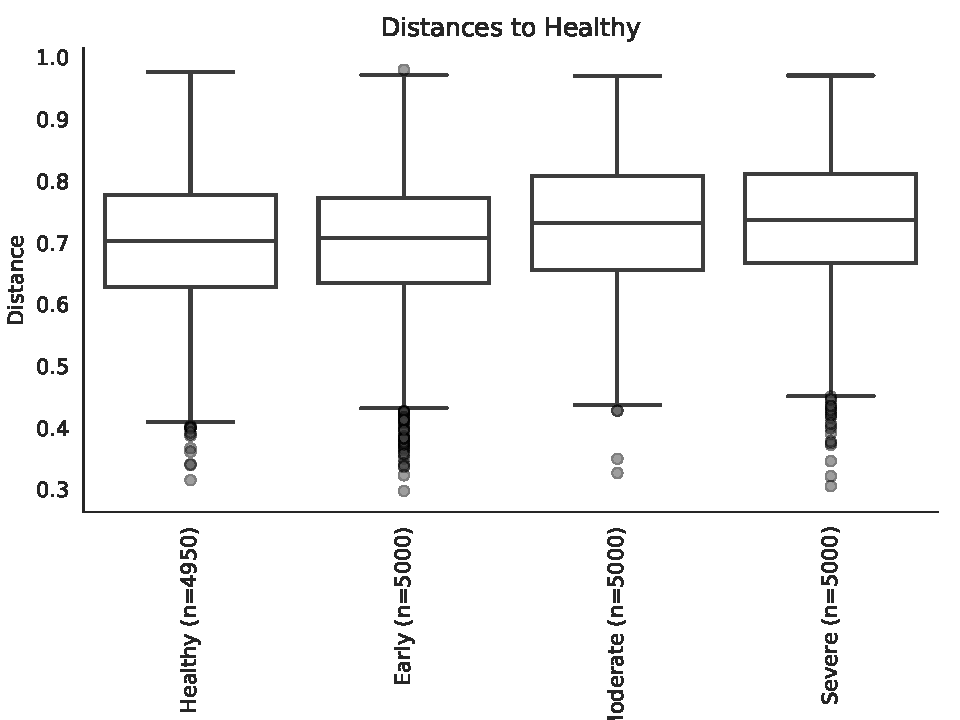
\includegraphics[width=0.4 \linewidth]{figures/BetaDiversity/Deblur/Bray/Healthy.pdf}
                    &
                    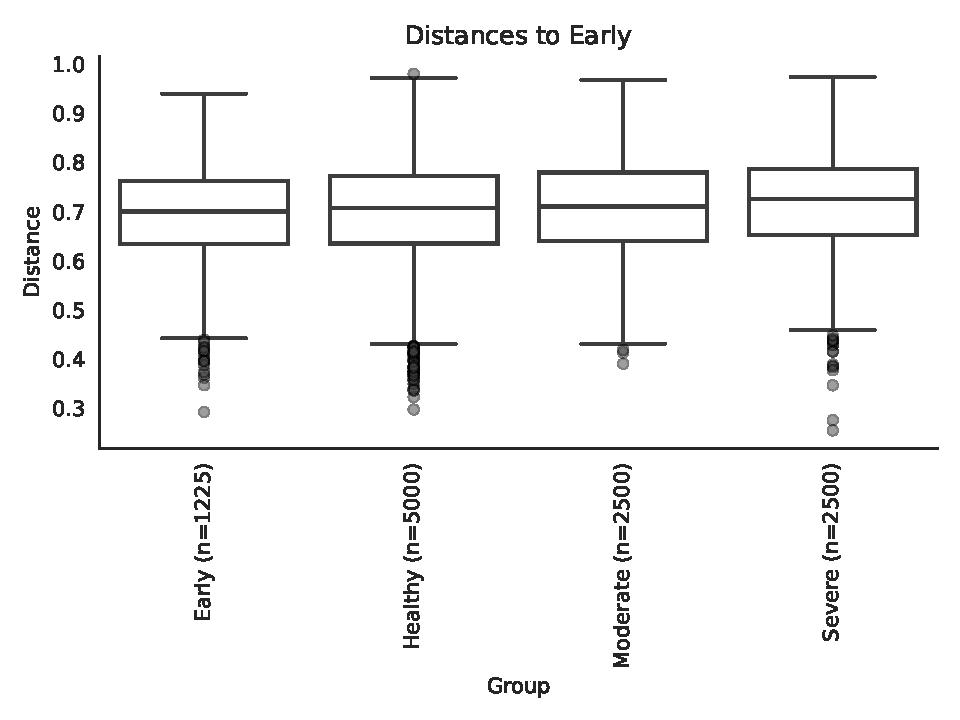
\includegraphics[width=0.4 \linewidth]{figures/BetaDiversity/Deblur/Bray/Early.pdf}
                    \\
                    \mbox{(a) Healthy} & \mbox{(b) Early} \\

                    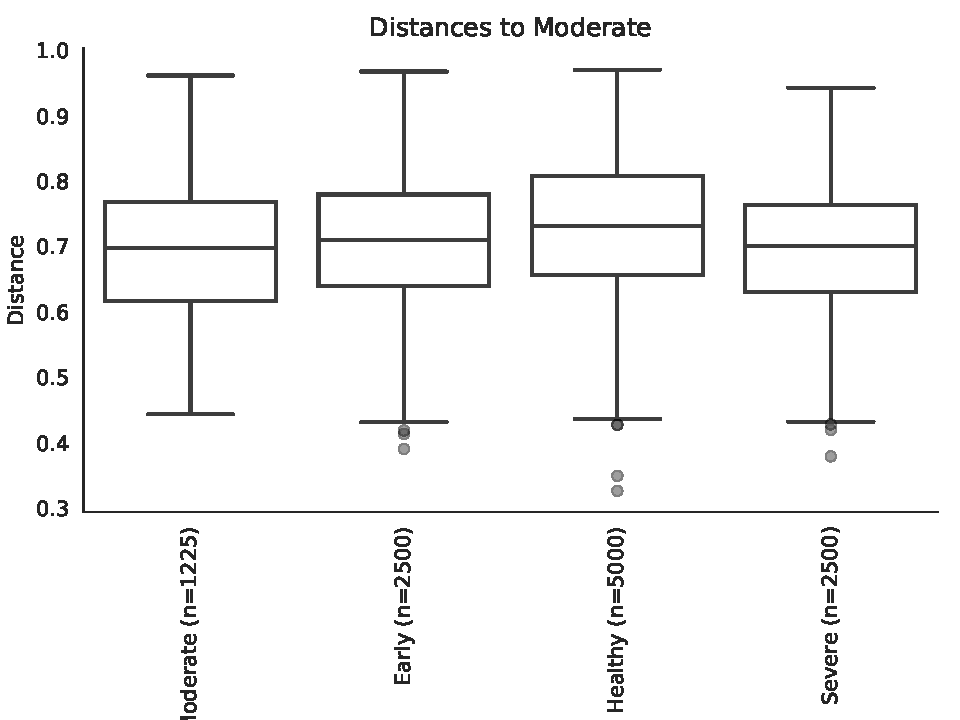
\includegraphics[width=0.4 \linewidth]{figures/BetaDiversity/Deblur/Bray/Moderate.pdf}
                    &
                    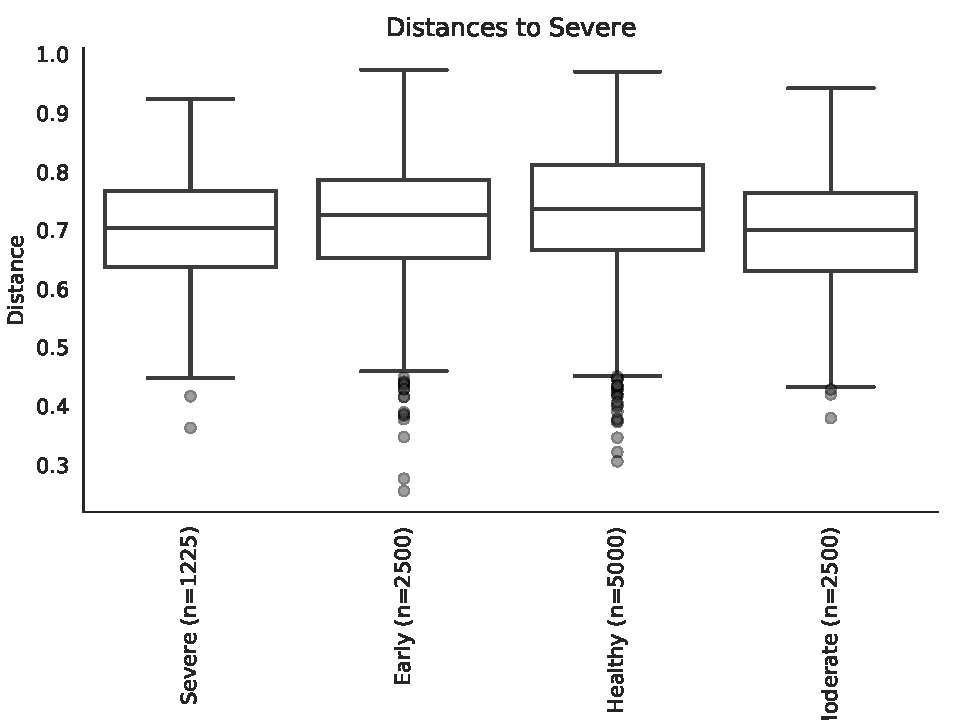
\includegraphics[width=0.4 \linewidth]{figures/BetaDiversity/Deblur/Bray/Severe.pdf}
                    \\
                    \mbox{(c) Moderate} & \mbox{(d) Severe} \\
                \end{array}$
                \caption{Bray-Curtis Distance Index with Deblur}
                \label{fig:bray-deblur}
            \end{figure}

            \begin{figure}[p]
                \centering
                $\begin{array}{cc}
                    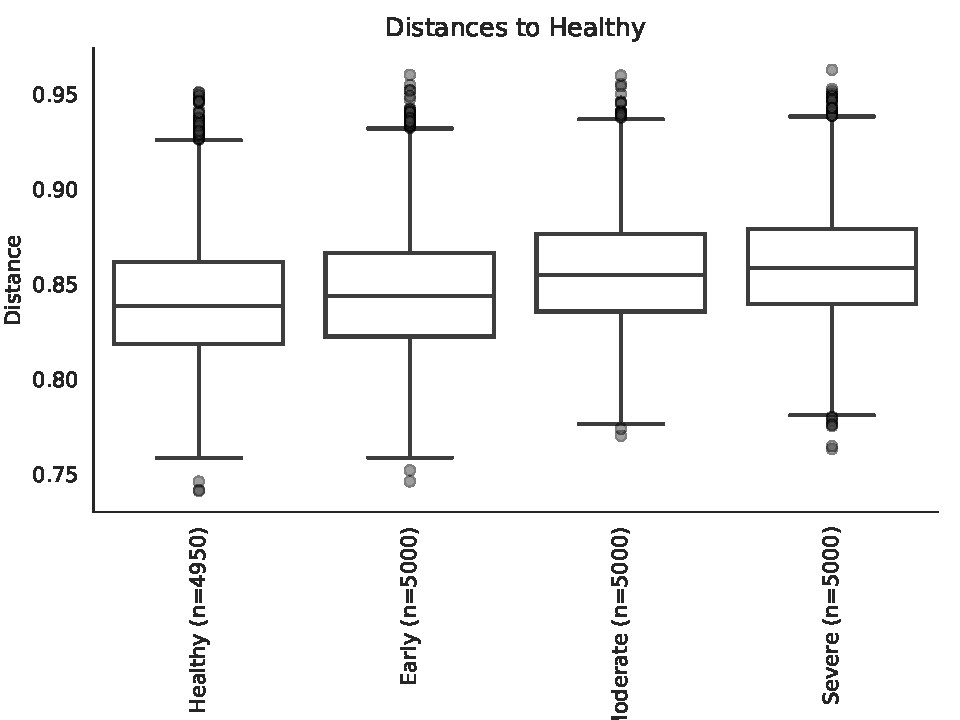
\includegraphics[width=0.4 \linewidth]{figures/BetaDiversity/Deblur/Jaccard/Healthy.pdf}
                    &
                    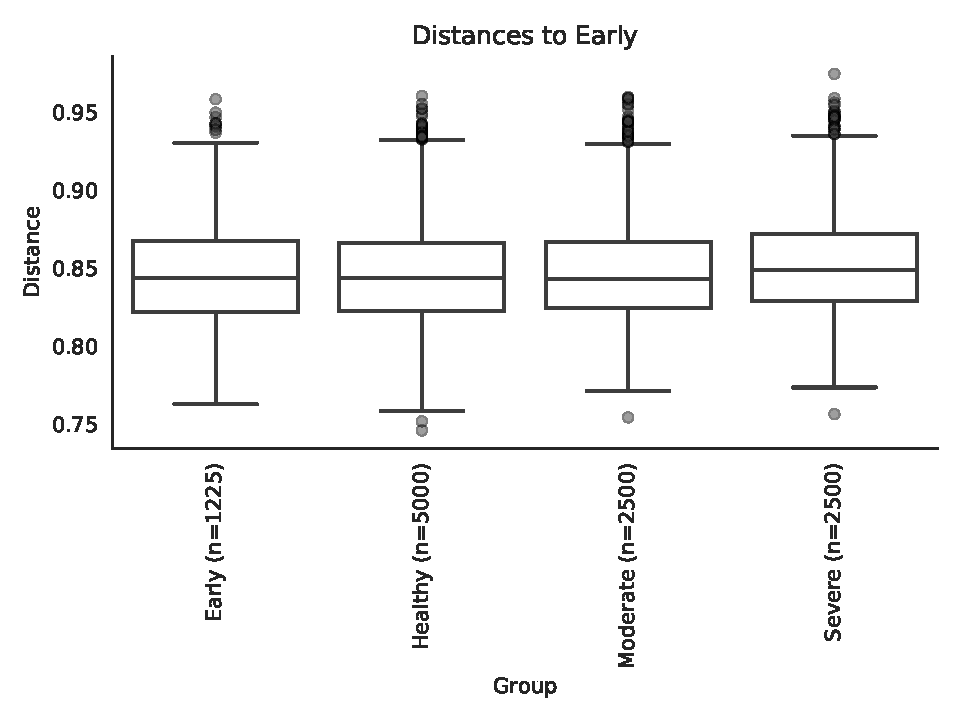
\includegraphics[width=0.4 \linewidth]{figures/BetaDiversity/Deblur/Jaccard/Early.pdf}
                    \\
                    \mbox{(a) Healthy} & \mbox{(b) Early} \\

                    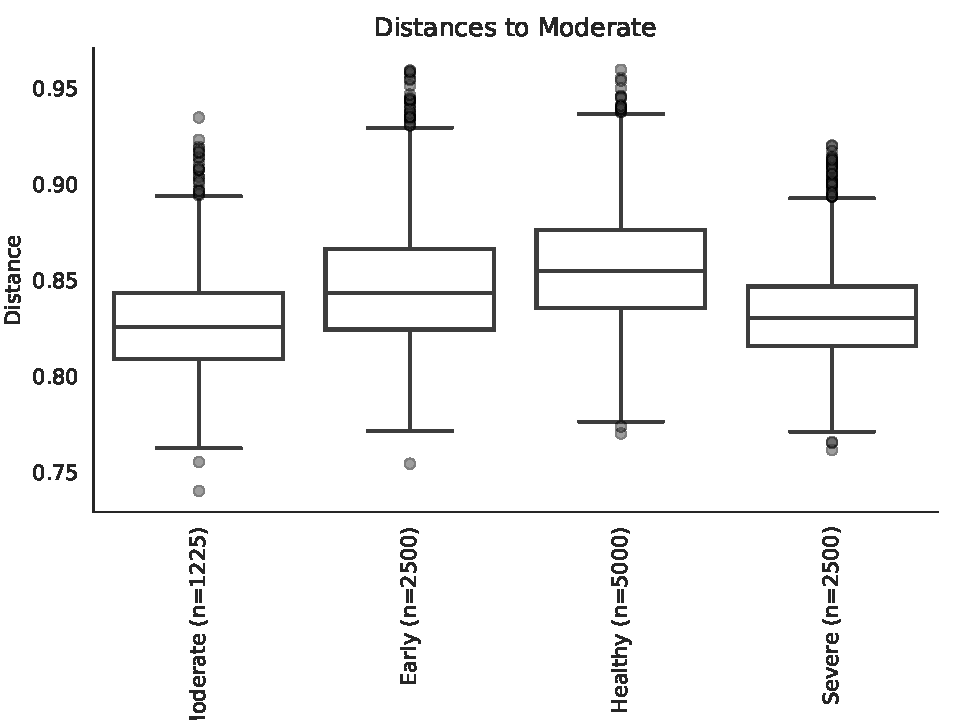
\includegraphics[width=0.4 \linewidth]{figures/BetaDiversity/Deblur/Jaccard/Moderate.pdf}
                    &
                    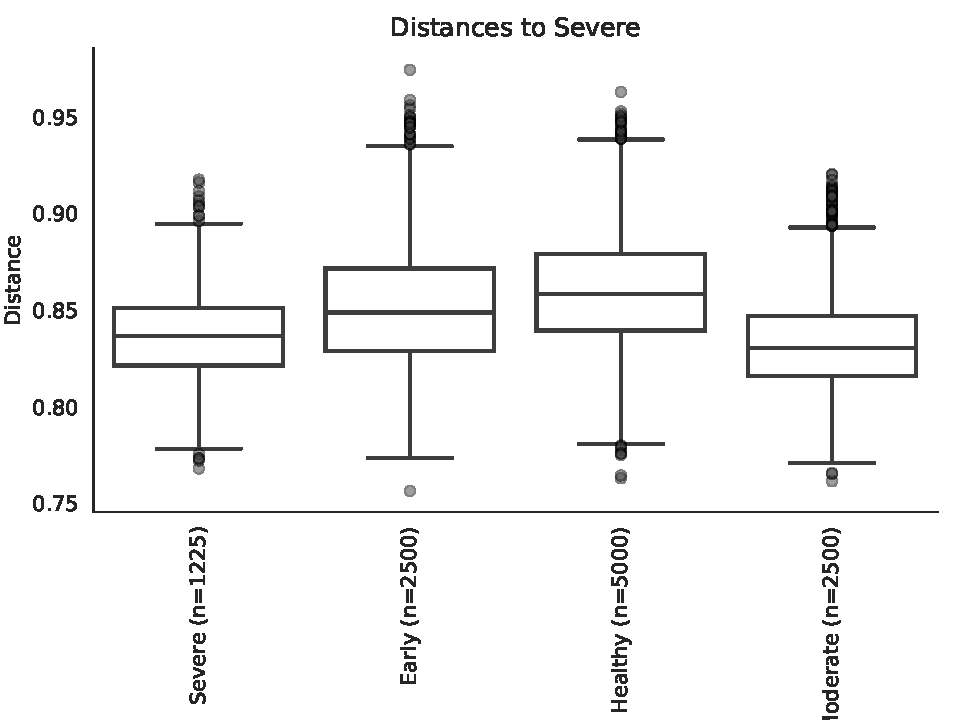
\includegraphics[width=0.4 \linewidth]{figures/BetaDiversity/Deblur/Jaccard/Severe.pdf}
                    \\
                    \mbox{(c) Moderate} & \mbox{(d) Severe} \\
                \end{array}$
                \caption{Jaccard Distance Index with Deblur}
                \label{fig:jaccard-deblur}
            \end{figure}

            \begin{figure}[p]
                \centering
                $\begin{array}{cc}
                    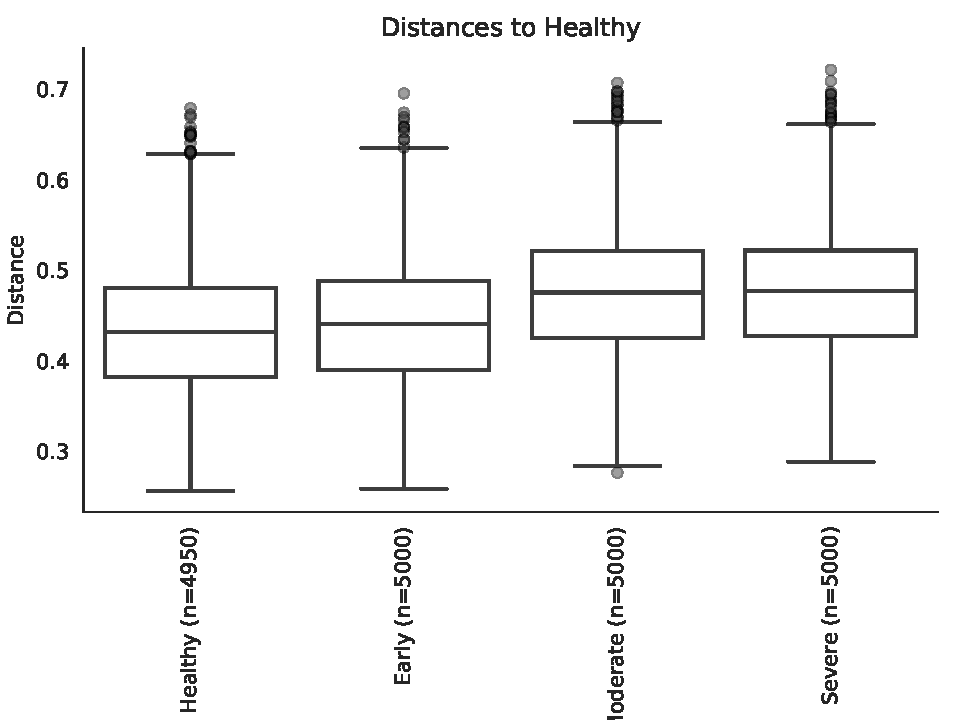
\includegraphics[width=0.4 \linewidth]{figures/BetaDiversity/Deblur/UnweightedUnifrac/Healthy.pdf}
                    &
                    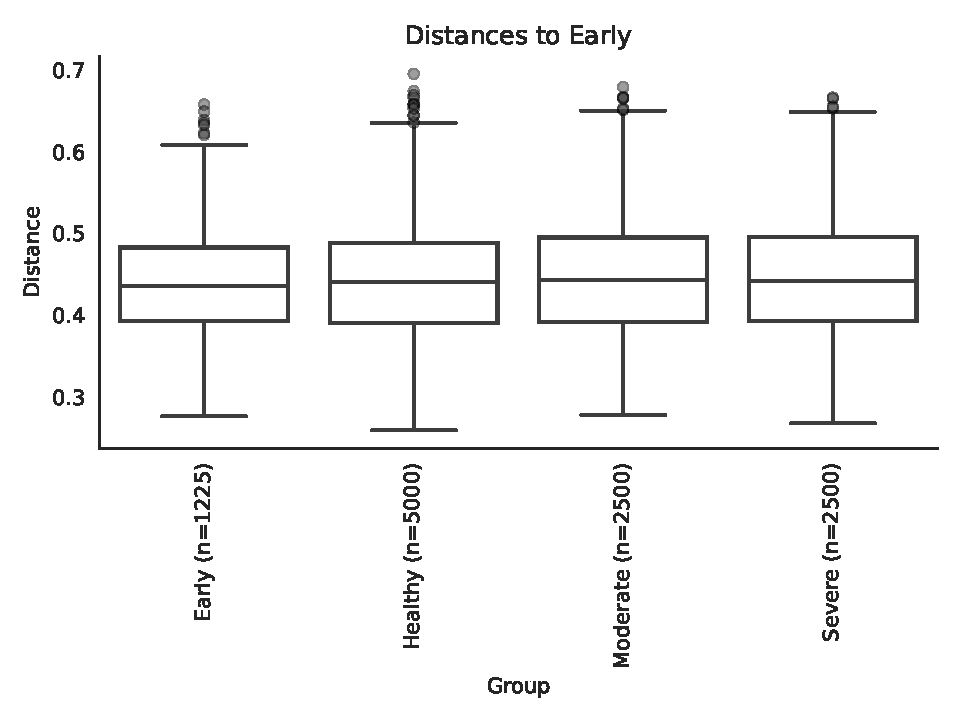
\includegraphics[width=0.4 \linewidth]{figures/BetaDiversity/Deblur/UnweightedUnifrac/Early.pdf}
                    \\
                    \mbox{(a) Healthy} & \mbox{(b) Early} \\

                    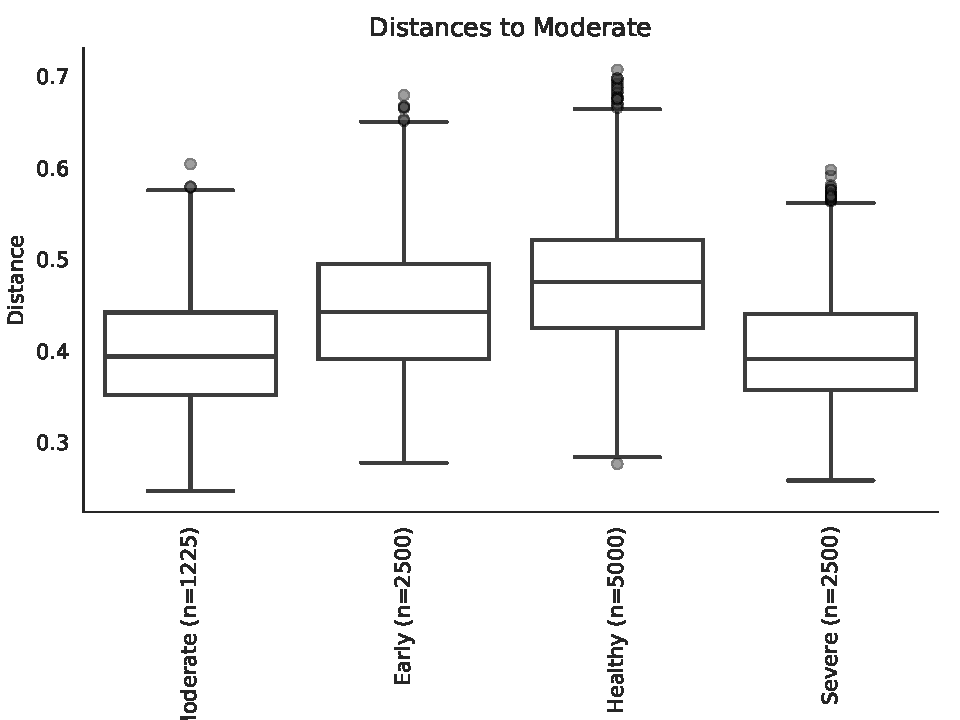
\includegraphics[width=0.4 \linewidth]{figures/BetaDiversity/Deblur/UnweightedUnifrac/Moderate.pdf}
                    &
                    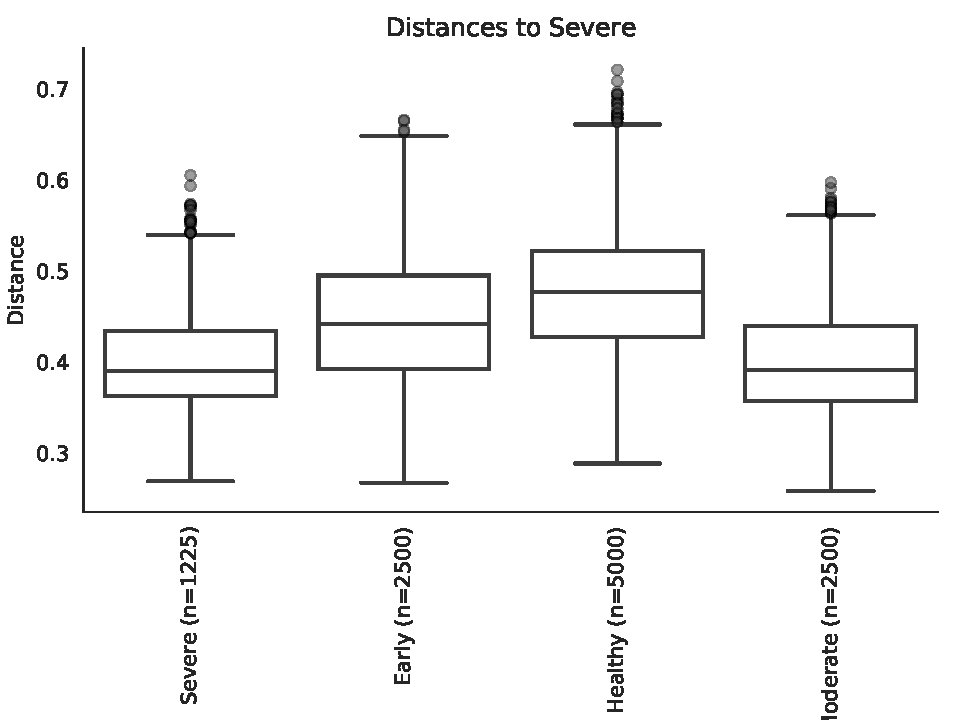
\includegraphics[width=0.4 \linewidth]{figures/BetaDiversity/Deblur/UnweightedUnifrac/Severe.pdf}
                    \\
                    \mbox{(c) Moderate} & \mbox{(d) Severe} \\
                \end{array}$
                \caption{Unweighted Unifrac Distance Index with Deblur}
                \label{fig:unweighted-deblur}
            \end{figure}

            \begin{figure}[p]
                \centering
                $\begin{array}{cc}
                    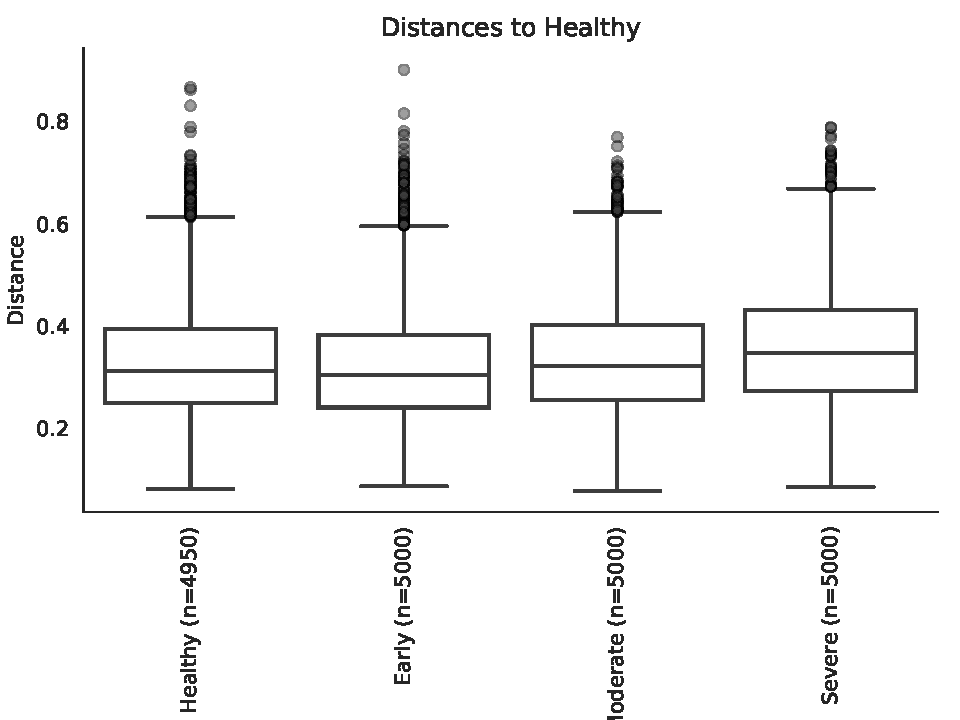
\includegraphics[width=0.4 \linewidth]{figures/BetaDiversity/Deblur/WeightedUnifrac/Healthy.pdf}
                    &
                    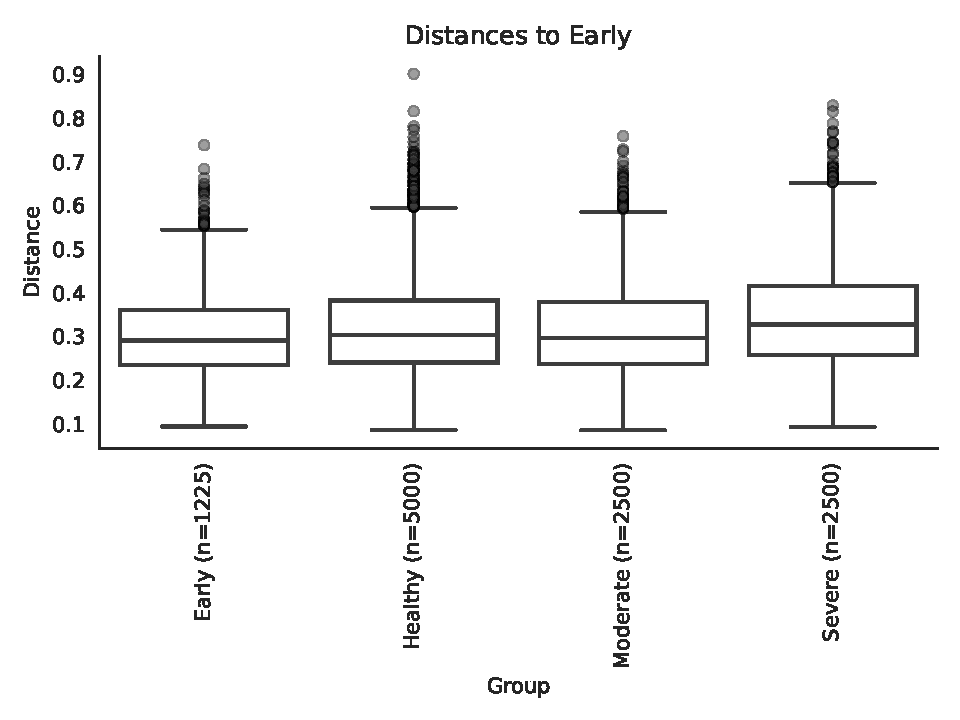
\includegraphics[width=0.4 \linewidth]{figures/BetaDiversity/Deblur/WeightedUnifrac/Early.pdf}
                    \\
                    \mbox{(a) Healthy} & \mbox{(b) Early} \\

                    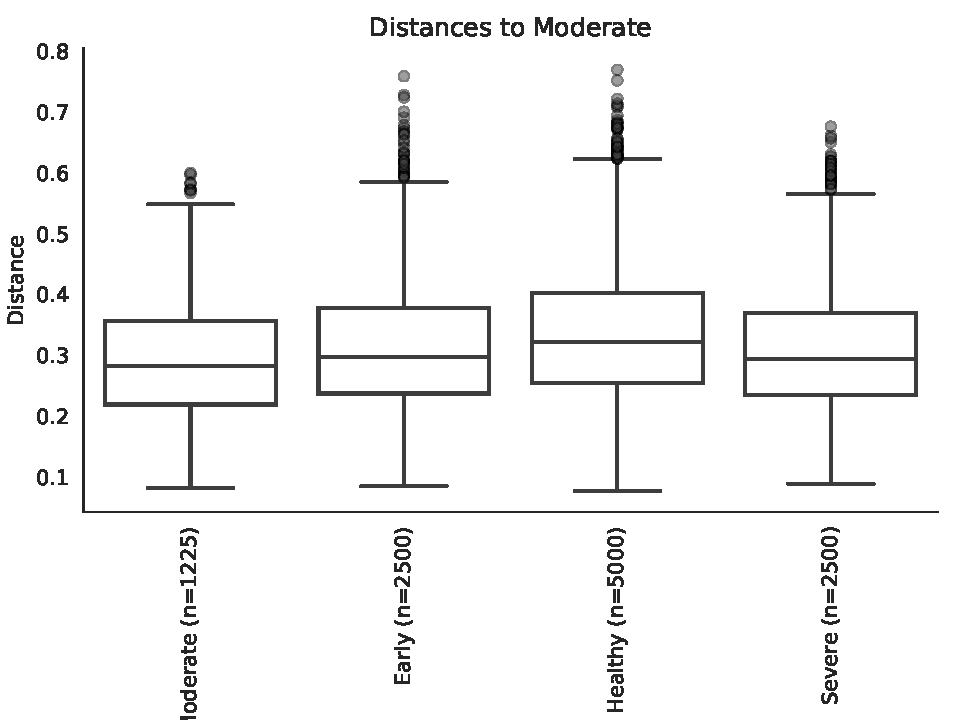
\includegraphics[width=0.4 \linewidth]{figures/BetaDiversity/Deblur/WeightedUnifrac/Moderate.pdf}
                    &
                    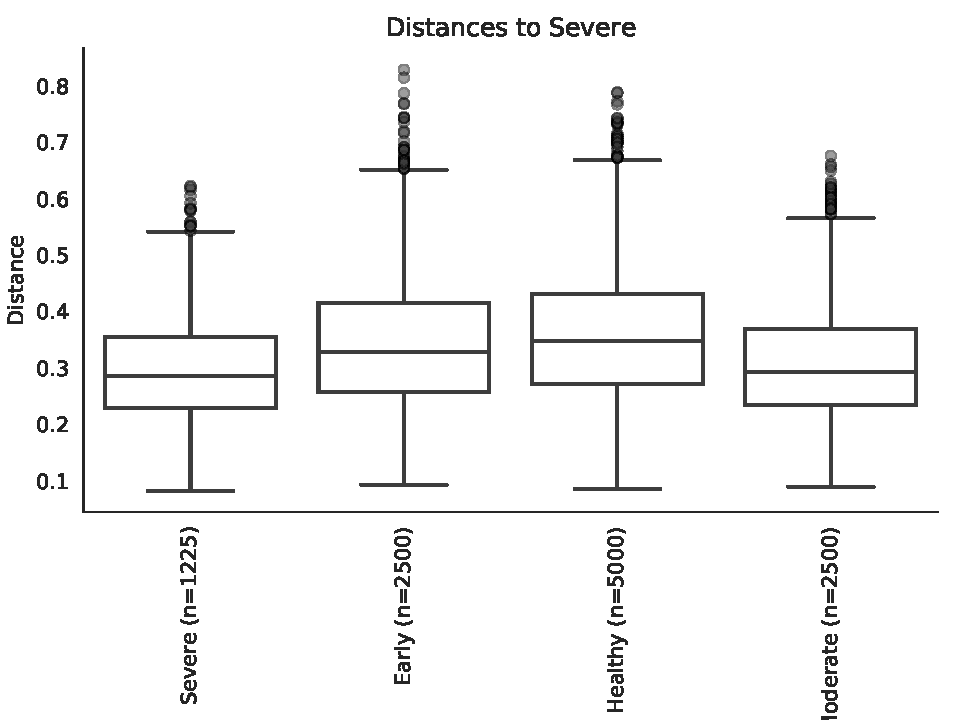
\includegraphics[width=0.4 \linewidth]{figures/BetaDiversity/Deblur/WeightedUnifrac/Severe.pdf}
                    \\
                    \mbox{(c) Moderate} & \mbox{(d) Severe} \\
                \end{array}$
                \caption{Weighted Unifrac Distance Index with Deblur}
                \label{fig:weighted-deblur}
            \end{figure}

        \subsection{ANCOM}

            \begin{table}[p]
                \centering
                \caption{ANCOM Significant Result with DADA2 and Greengenes}
                \label{tb:ANCOM-dada2-gg}

                \csvreader[tabular=p{10cm}cc, nohead, column count=3, table head=\hline, late after first line=\\\hline, table foot=\hline, respect underscore]{csv/ANCOM/DADA2.gg.csv}{}{\csvlinetotablerow}
            \end{table}

            \begin{figure}[p]
                \centering
                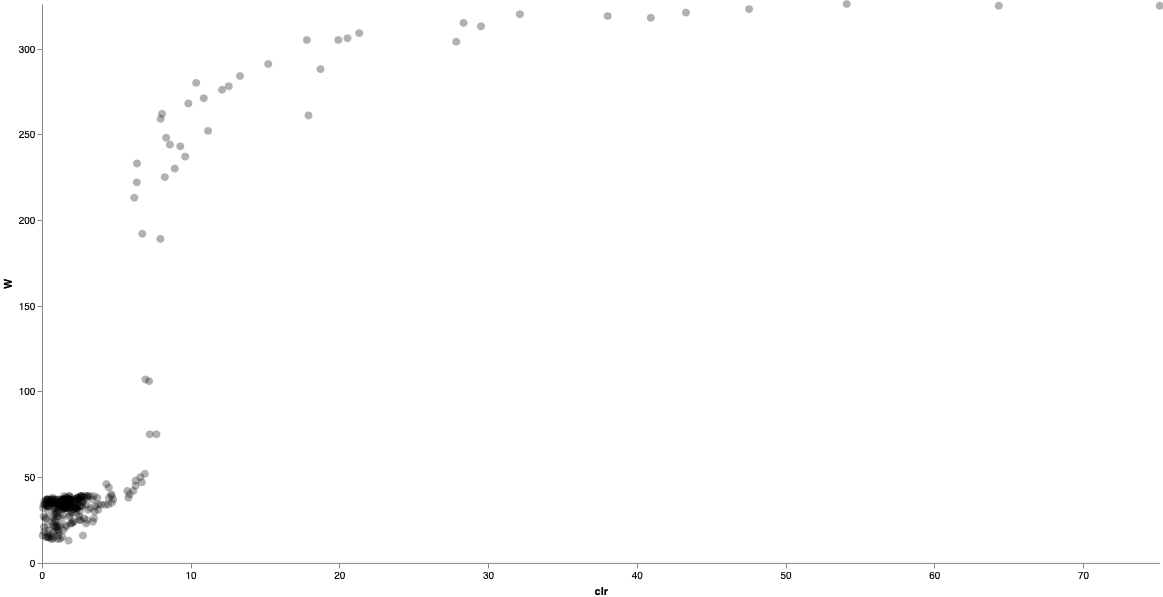
\includegraphics[width=0.8 \linewidth]{figures/ANCOM/DADA2.gg.png}
                \caption{ANCOM Volcano Plot with DADA2 and Greengenes}
                \label{fig:volcano-dada2-gg}
            \end{figure}

            \begin{table}[p]
                \centering
                \caption{ANCOM Significant Result with DADA2 and SILVA}
                \label{tb:ANCOM-dada2-silva}

                \csvreader[tabular=p{10cm}cc, nohead, column count=3, table head=\hline, late after first line=\\\hline, table foot=\hline, respect underscore]{csv/ANCOM/DADA2.silva.csv}{}{\csvlinetotablerow}
            \end{table}

            \begin{figure}[p]
                \centering
                \includegraphics[width=0.8 \linewidth]{figures/ANCOM/DADA2.silva.png}
                \caption{ANCOM Volcano Plot with DADA2 and SILVA}
                \label{fig:volcano-dada2-silva}
            \end{figure}

            \begin{table}[p]
                \centering
                \caption{ANCOM Significant Result with Deblur and Greengenes}
                \label{tb:ANCOM-deblur-gg}

                \csvreader[tabular=p{10cm}cc, nohead, column count=3, table head=\hline, late after first line=\\\hline, table foot=\hline, respect underscore]{csv/ANCOM/Deblur.gg.csv}{}{\csvlinetotablerow}
            \end{table}

            \begin{figure}[p]
                \centering
                \includegraphics[width=0.8 \linewidth]{figures/ANCOM/Deblur.gg.png}
                \caption{ANCOM Volcano Plot with Deblur and Greengenes}
                \label{fig:volcano-deblur-gg}
            \end{figure}

            \begin{table}[p]
                \centering
                \caption{ANCOM Significant Result with DADA2 and SILVA}
                \label{tb:ANCOM-deblur-silva}

                \csvreader[tabular=p{10cm}cc, nohead, column count=3, table head=\hline, late after first line=\\\hline, table foot=\hline, respect underscore]{csv/ANCOM/DADA2.silva.csv}{}{\csvlinetotablerow}
            \end{table}

            \begin{figure}[p]
                \centering
                \includegraphics[width=0.8 \linewidth]{figures/ANCOM/Deblur.silva.png}
                \caption{ANCOM Volcano Plot with Deblur and SILVA}
                \label{fig:volcano-deblur-silva}
            \end{figure}

    \section{Discussion}

    \bibliographystyle{apacite}
    \bibliography{reference}
\end{document}